\documentclass[aip,jcp,a4paper,11pt]{revtex4-1}
%\documentclass[draft]{revtex4-1}
\usepackage[utf8x]{inputenc}
\usepackage{amsmath}
\usepackage{amsfonts}
\usepackage{amssymb}
\usepackage{bm}
\usepackage{color}
\usepackage{graphicx}
\usepackage{booktabs}
\usepackage{array}
%\usepackage{subfigure}
\usepackage{epsfig,subfig,graphicx}
\usepackage{booktabs}
\usepackage{multirow}

\newcommand{\two}{0.475\textwidth}
\newcommand{\three}{0.31\textwidth}

\newlength\tbspace
\setlength\tbspace{5mm}
\newcolumntype{R}{r<{\hspace{\tbspace}}}
\newcolumntype{A}{r<{\hspace{2.5mm}}}
\newcommand{\bn}{\mathbf{n}}
\newcommand{\br}{\mathbf{r}}
\newcommand{\bs}{\mathbf{s}}
\newcommand{\bv}{\mathbf{v}}
\newcommand{\bx}{\mathbf{x}}
\newcommand{\by}{\mathbf{y}}
\newcommand{\bR}{\mathbf{R}}
\newcommand{\bP}{\mathbf{P}}
\newcommand{\bh}{\mathbf{h}}
\newcommand{\bG}{\mathbf{G}}
\newcommand{\cA}{\mathcal{A}}
\newcommand{\cN}{\mathcal{N}}
\newcommand{\cI}{\mathcal{I}}
\newcommand{\cS}{\mathcal{S}}
\newcommand{\cD}{\mathcal{D}}
\newcommand{\cR}{\mathcal{R}}
\newcommand{\sR}{\mathbb{R}}
\newcommand{\bTh}{\bm{\Theta}}
\newcommand{\bXi}{\bm{\Xi}}

\newcommand{\App}{{\widehat{\Phi}_{j,\varepsilon}}}
\newcommand{\GApp}{{\widehat{\Phi}_{\varepsilon}}}
\newcommand{\FApp}{{\widehat{f}_{j,\varepsilon}}}
\newcommand{\GFApp}{{\widehat{f}_{\varepsilon}}}
\newcommand{\AppZ}{{\widehat{\Phi}^0_{j}}}
\newcommand{\GAppZ}{{\widehat{\Phi}^0}}
\newcommand{\red}{\color{red}}
\newcommand{\black}{\color{black}}
\newcommand{\nablai}{\nabla_{\!i}\,}
\newcommand{\Di}{D_i}
\newcommand{\nablaj}{\nabla_{\!j}\,}
\newcommand{\nablak}{\nabla_{\!k}\,}
\newcommand{\Dj}{D_j}

\newcommand{\Best}[1]{\color{red}{\tt #1}\color{black}}
%opening

\begin{document}
\title{Computation of Forces arising from the Polarizable Continuum Model within the Domain-Decomposition Paradigm}

\author{Paolo Gatto}
\affiliation{Mathematics Division, Center for Computational Engineering Science, RWTH Aachen University, Aachen, Germany}

\author{Filippo Lipparini}
\email{filippo.lipparini@unipi.it}
\affiliation{Dipartimento di Chimica e Chimica Industriale, Universit\`a di Pisa, Via G. Moruzzi 13, 56124 Pisa, Italy}


\author{Benjamin Stamm}
\email{best@mathcces.rwth-aachen.de}
\affiliation{Mathematics Division, Center for Computational Engineering Science, RWTH Aachen University, Aachen, Germany}



\begin{abstract}
The domain decomposition (dd) paradigm, originally introduced for the Conductor-like Screening Model (COSMO), has been recently extended to the dielectric Polarizable Continuum Model (PCM), resulting in the ddPCM method. We present here a complete derivation of the analytical derivatives of the ddPCM energy with respect to the positions of the solute's atoms, and discuss their efficient implementation. As it is the case for the energy, we observe a quadratic scaling, which is discussed and demonstrated with numerical tests.  
%Within implicit solvation models, the domain-decomposition strategy for the computation of the electrostatic energy due to the solvent based on the Polarizable %Continuum Model (PCM) has recently been developed. 
%The methodological development started with the so-called ddCOSMO method and has recently be generalized to the PCM equation resulting in the ddPCM-method [Stamm {\it et al.}, J. Chem. Phys. 144, 054101 (2016)] for which derive the forces within this article. 
%We show the derivation of the forces and derive an efficient implementation followed by numerical tests.
%In our previous work we developed a Schwarz's domain decomposition method for the Polarizable Continuum Model (PCM) equation. The discretization is systematically improvable and fully consistent with the Conductor-like Screening Model (COSMO), in the sense that it reduces to COSMO for large dielectric constants. In this work, we build on top of this framework and introduce the computation of analytical forces.

\end{abstract}

\maketitle


\section{Introduction}\label{sec:intro}
Solvation plays a crucial role in many processes in chemistry and biochemistry. As a consequence, including the effects of the solvent in the description of a chemical system is of paramount importance in computational chemistry. In principle, this can be achieved by including sufficiently many solvent molecules in the computational representation of the system. Unfortunately, solute-solvent interactions are often dominated by long-range electrostatic contributions, which would require the inclusion of an extended number of solvent molecules to be properly described. When an accurate, quantum mechanical level of theory is employed, the presence of a large number of solvent molecules can easily make the computation very expensive, or even completely unfeasible. Furthermore, the system would not be correctly represented by a single configuration, thus requiring  to repeat the computation many times in order to take care of statistical sampling. 

Such a brute force strategy is not only undesirable, but also unnecessary when one's aim is to describe the solute and its properties in the presence of a solvent, rather than the solvent itself. In such case, a \textit{focused model} can be used, where the solute is described accurately, while the solvent is treated with an approximated level of theory which is, however, sufficient to introduce the desired solute-solvent interactions. 
A popular choice to describe solvation is to use QM/MM models\cite{Warshel_JMB_QMMM,Warshel_JACS_QMMM,Gao_Science_QMMM,Bakowies_JPC_QMMM,Truhlar_TCA_QMMMReview,Thiel_ACIE_QMMMReview,
Barone_Libro_QMMM,Morokuma_CR_ONIOM,Cappelli_IJQC_FQRev}, where the solute is treated at a quantum mechanical level of theory, while the solvent is described with a force field, and solute-solvent interactions are introduced via electrostatic interactions, possibly including mutual polarization\cite{Curutchet_JCTC_MMPol,Kongsted_JCTC_MMPExc,Christiansen_JCTC_MMPExcCCDFT,Steindal_PCCP_MMPExc,Caprasecca_JCTC_FMM,Lipparini_JCP_FQMag,Lipparini_JCTC_FQTD,Boulanger_JCTC_Drude,Boulanger_JCTC_QMMMPolPCM,Loco_JCTC_QMAMOEBA}. However, QM/MM methods still require to take care of the statistical sampling, which, when interested in certain properties, can be particularly challenging\cite{Lipparini_JCTC_ORMoxy,Giovannini_JCTC_FQVCD,Giovannini_JCTC_FQROA}.

Polarizable Continuum Solvation Models\cite{MST,ReviewPCM_1994,ReviewPCM_2005,Orozco_CR_Solvent00,Klamt:2011we,Mennucci:2012ct,honig1995cla,Roux:1999vp} (PCSM's) replace the solvent with a uniform, infinite, and polarizable continuum, which interacts with the solute's density of charge in a mutually polarizable fashion. PCSM's do not require statistical sampling, as such an effect is implicitly included in the use of a macroscopic property, namely the bulk dielectric permittivity $\varepsilon_s$, to model the solvent response. The interaction between the solute and the solvent is modeled via electrostatics. For a given value of the solute's density of charge, the electrostatics equations are solved in the presence of the polarizable continuum and a \emph{reaction potential} is then added to the solute's Hamiltonian. A new density of charge is then computed and the process is iterated until mutual polarization has been achieved\cite{ReviewPCM_2005,Lipparini_JCP_VPCM,Lipparini_JCTC_VPCMSCF,Lipparini_JCP_Perspective}.
Over the last decades, PCSM's have been extended to introduce solvent effects on molecular structures and properties\cite{Tomasi_PCCP_PCMProps,Mennucci_Chir_PCMProps,Mennucci_JPCL_PCM}, and are nowadays available in most quantum Chemistry codes, to the extent that have become a standard tool among computational chemists. 

More recently, PCSM's and QM/MM methods have been combined\cite{Pedone_CPC_QMMMPCM,Rega_JACS_QMMMPCM,Vreven_JCP_OniomPCM,Bandyopadhyay2002,Lipparini_JCTC_FQPCM,Caprasecca_JCTC_FMM,Steindal_JCPA_QMMMPCM,Boulanger_JCTC_QMMMPolPCM,Caprasecca_JCTC_QMMMPolPCM} in order to retain the atomistic description provided by QM/MM models, which is needed in order to describe specific solute-solvent interactions, and the inexpensive handling of long-range electrostatic interactions of PCSM's.

Standard implementations of PCSM's usually employ the Boundary Element Method\cite{MST,ReviewPCM_1994,ReviewPCM_2005,Scalmani_JCP_CSC,York_JPCA_CSC,
Herbert_JCP_ISWIG} (BEM) to numerically solve a discretized integral equation. This requires the solution of a linear system whose size scales linearly, although with a large proportionality constant, with respect to the number of atoms. This task is usually carried out through standard dense linear algebra techniques, such as the LU decomposition\cite{Cammi_JCC_Inversion}, which require a computational effort of cubic complexity, with respect to the size of the system. Consequently, the solution step can rapidly become demanding when dealing with systems as large as those treated via QM/MM methods, and one should seek other strategies. An alternative is provided by iterative techniques, which reduce the computational cost to that of several matrix-vector multiplications\cite{Scalmani_TCA_Iterative}, which is, in  the general case, quadratic. When fast summation techniques, e.g., the Fast Multipole Method (FMM)\cite{FMM}, can be employed, the computational complexity can be further reduced. Thus, it is possible to solve the PCSM linear equations in a number of floating point operations which is linear with respect to the number of atoms. Nevertheless, the solution of the PCSM equations can still represent a formidable bottleneck for large systems\cite{Lipparini_JPCL_ddCOSMO}, especially when repeated computations are required for statistical sampling purposes or time-dependent simulations.

In recent years, we have proposed an alternative approach for PCSM's which is based on  domain-decomposition. We introduced a novel strategy\cite{Cances_JCP_ddCOSMO}, referred to as ddCOSMO\cite{Cances_JCP_ddCOSMO,Lipparini_JCTC_ddCOSMO,Lipparini_JPCL_ddCOSMO,Lipparini_JCP_ddCOSMO-QM}, to solve the PCSM equation for the Conductor-like Screening Model\cite{Klamt_JCS_Cosmo} (COSMO) in combination with Van der Waals molecular cavities. \color{red}COSMO approximates the solution to Poisson's equation for a density of charge embedded in a dielectric continuum by introducing an approximated boundary condition known as the scaled conductor boundary condition. As a consequence, the electrostatics treatment is greatly simplified, while retaining, thanks to the empirical scaling, a good accuracy also for non-polar solvents\cite{Klamt_JCTC_COSMOBench}.\color{black}
As a first step, the COSMO equation in its differential form is rewritten as a system of coupled linear differential equations on each sphere, where the coupling occurs only between overlapping spheres. Secondly, each differential equation is recast as an integral equation, so that it can be efficiently solved by using a (truncated) expansion of spherical harmonics\cite{Cances_JCP_ddCOSMO}. \color{red}Thanks to the COSMO approximate boundary condition,\color{black} the discretization produces a block-sparse linear system\cite{Lipparini_JCTC_ddCOSMO}, where only the blocks corresponding to overlapping spheres are nonzero. This structure allows for a computational cost that scales linearly with respect to the number of atoms, and is overall very small as compared to competing techniques. Indeed, as shown in ref. \citenum{Lipparini_JPCL_ddCOSMO}, as many as two or three orders of magnitude are gained by the ddCOSMO approach.

More recently, the method has been generalized to the Integral Equation Formalism Polarizable Continuum Model (IEFPCM) equation\cite{Mennucci_JCP_IEF1,Mennucci_JMC_IEF2,Mennucci_JPCB_IEF3}, \color{red}which solves Poisson's equation for a solute inside a dielectric without approximating the boundary condition.\color{black} This resulted in the ddPCM method\cite{Stamm_JCP_DDPCM}, which is based on the same domain-decomposition approach. 
While the method has been developed in \cite{Stamm_JCP_DDPCM} to compute the electrostatic contribution to the solvation energy, the aim of this article is to present the derivation of analytical forces of the ddPCM solvation energy.

This paper is organized as follows. Section \ref{sec:review} reviews the ddPCM and ddCOSMO methods that we have previously developed. In Section \ref{sec:forces} we describe the derivation of the ddPCM forces and discuss their efficient implementation. Section \ref{sec:experiments} is devoted to numerical experiments. Finally, in Section \ref{sec:conclusions} we draw conclusions from the presented work and point to possible future directions of research.

\section{A Brief Review of the ddPCM Strategy}\label{sec:review}

\subsection{The Polarizable Continuum Model}
In PCSM's, the solute is accommodated in a hollow molecular cavity $\Omega$ surrounded by the continuum, which can be treated either as a conductor, as in COSMO, or as a dielectric, as in PCM. We follow the customary approach of taking the cavity to be the so-called Van der Waals cavity\cite{ReviewPCM_2005}, i.e., the union of spheres centered at each atom with radii coinciding with (scaled) van der Waals radii. Note that the similar Solvent Accessible Surface (SAS) cavity can be treated through this approach as well. Models based on the Solvent Excluded Surface (SES) have recently been proposed~\cite{Harbrecht2011,quan2017polarizable,C5CP03410H,JCC:JCC21431}, however are not considered here.

The electrostatic part of the solute/solvent interaction is given by the electrostatic interaction energy between the solute's density of charge $\rho$ and the polarization potential of the solvent $W$, namely
\[
E_s = \tfrac{1}{2}\, f(\varepsilon_s)\,\int_\Omega \rho(x) W(x) \, dx,
\]
Here $f(\varepsilon_s)$ is an empirical scaling that depends on the dielectric constant $\varepsilon_s$ of the solvent, e.g., $f(\varepsilon_s) = (\varepsilon_s - 1)/(\varepsilon_s + x)$ for COSMO, \color{red}where $x$ is an empirical parameter\color{black}, and $f(\varepsilon_s) = 1$ for PCM, $\rho$ is the solute's charge density, and $W$ is the polarization potential of the solvent. The quantities $W$ and $E_s$ are usually referred to as the reaction potential and the electrostatic contribution to the solvation energy, respectively. 

The reaction potential is defined as $W = \varphi - \Phi$, where $\varphi$ is the total electrostatic potential of the solute/solvent system and $\Phi$ is the potential of the solute \emph{in vacuo}. In the case of the PCM, the total potential $\varphi$ satisfies the generalized Poisson equation\cite{Mennucci_JCP_IEF1,Mennucci_JMC_IEF2}
\begin{equation}
 \label{eq:genpoisson}
\text{div} \, (\varepsilon \, \nabla \varphi) = -4\pi \rho,
\end{equation}
where the coefficient $\varepsilon$ is defined as $\varepsilon(x) = 1$ when $x \in \Omega$, and $\varepsilon(x) = \varepsilon_s$ otherwise. As a consequence, the reaction potential fulfills
\begin{equation} 
\label{eq:pcmpde}
\left \{ 
\begin{alignedat}{4}
\Delta \,  W &= 0  &&\mbox{in } \sR^3\setminus \Gamma  \\
 \ [\![W]\!] &= 0  &&\mbox{on } \Gamma\\
\  [\![\varepsilon \, \partial_n W]\!] &= (\varepsilon_s-1)\, \partial_n \Phi &\qquad& \mbox{on } \Gamma.
\end{alignedat} 
\right.
\end{equation}
Here $\Gamma=\partial\Omega$ is the boundary of the cavity, $\partial_n$ is the normal derivative at $\Gamma$, and $[\![\,\cdot\,]\!]$ is the jump operator (inside minus outside) at $\Gamma$.

The reaction potential $W$ is a \emph{single-layer potential}, and can be represented\cite{sauter2010boundary} as $W(x) = (\tilde{\mathcal{S}}\sigma)(x)$ when $x \in \sR^3 \setminus \Gamma$, or $W(s) = (\mathcal{S}\sigma)(s)$ when $s \in \Gamma$, where we introduced a surface density of charge $\sigma$ usually referred to as \emph{apparent surface charge}. The integral operators
\begin{equation*}
 %\label{eq:Stilde}
 (\tilde{\cS}\sigma)(x) = \int_{\Gamma} \frac{\sigma(t)}{|x-t|} \, dt \qquad  x \in \sR^3 \setminus \Gamma \qquad , \qquad  ({\cS}\sigma)(s) = \int_{\Gamma} \frac{\sigma(t)}{|s-t|} \, dt \qquad  s \in \Gamma
\end{equation*}
are known, respectively, as the single layer potential and the single layer operator. Furthermore, the latter one is invertible\cite{Calderon}. It can be shown that $\sigma$ satisfies the equation $\sigma = 1/4\pi \, [\![ \partial_n W]\!]$, so that it is possible to recast the PCM problem \eqref{eq:pcmpde} as a single integral equation for $\sigma$. Let $\cD$ be the double layer operator
\begin{equation}\label{eq:DOper}
 ({\cD}\sigma)(s) = \int_{\Gamma} \sigma(t) \, \partial_{n(t)} \bigg( \frac{1}{|s-t|}\bigg) \,dt \qquad s \in \Gamma
\end{equation}
and define the operators 
\begin{equation}
 \label{eq:Reps}
 \cR_\varepsilon = 2\pi \, g(\varepsilon_s) \, \cI - \cD \qquad, \qquad \cR_\infty = 2\pi \, \cI - \cD
\end{equation}
where $g(\varepsilon_s) = (\varepsilon_s+1)/(\varepsilon_s-1)$ and $\cI$ is the identity. It can be shown\cite{ReviewPCM_2005} that the apparent surface charge satisfies
\begin{equation}
\label{eq:IEFPCM}
\cR_\varepsilon \, \cS \, \sigma = - \cR_\infty \, \Phi \qquad \text{on }\Gamma
\end{equation}
This is known as the IEF-PCM equation, and it involves the operators $\cR_\infty$ and $\cR_\varepsilon$, which are both invertible. When the dielectric constant $\varepsilon_s$ approaches infinity, the IEF-PCM equation simplifies to $\cS \, \sigma = - \Phi$ on $\Gamma$, which is the Integral Equation Formulation of the Conductor-like Screening Model (COSMO)\cite{Lipparini_JCP_VPCM}.


\subsection{The ddPCM-method}


We recall how to solve the IEF-PCM boundary integral equation \eqref{eq:IEFPCM} within the domain-decomposition paradigm. As a preliminary step, we set $\Phi_\varepsilon = \cS \, \sigma$ and write \eqref{eq:IEFPCM} as a succession of two integral equations, the latter of which is equivalent to the COSMO equation\cite{Cances_Librone_PCM}, namely
\begin{alignat}{3}
\cR_\varepsilon \, \Phi_\varepsilon & = \cR_\infty \, \Phi \qquad && \text{on }\Gamma  \label{eq:ddPCM-1} \\
\cS \, \sigma & = -\Phi_\varepsilon  && \text{on }\Gamma \label{eq:ddPCM-2} 
\end{alignat}
Indeed, \eqref{eq:ddPCM-2} is a COSMO equation with the modified potential $\Phi_\varepsilon$ in place of the potential $\Phi$. This allows to develop the ddPCM strategy as an extension of the ddCOSMO approach. First, equation \eqref{eq:ddPCM-1} is solved in order to compute the right-hand-side $-\Phi_\varepsilon$ of equation \eqref{eq:ddPCM-2}; secondly, ddCOSMO is employed to solve equation \eqref{eq:ddPCM-2} with the modified potential $-\Phi_\varepsilon$, and compute the solvation energy $E_s$.


In order to discuss the domain-decomposition approach employed for both steps, let us introduce some notation. As anticipated, we take the cavity $\Omega$ be the union of $M$ spheres $\Omega_j = B(x_j, r_j)$ with boundaries $\Gamma_j$. We define $\Gamma_j^\text{ext}:= \Gamma_j \cap \Gamma$ and $\Gamma_j^\text{int} := \Gamma_j \cap \Omega$, as the portion of the surface $\Gamma_j$ which is exposed to the solvent or buried into the cavity, respectively, and let $U_j: \Gamma_j \to \mathbb{R}$ be the characteristic function of $\Gamma_j^\text{ext}$. Let $\Phi_j : \Gamma_j \to \mathbb{R}$ and $\Phi_{\varepsilon,j} : \Gamma_j \to \mathbb{R}$ be, respectively, the local trivial extensions of $\Phi$ and $\Phi_\varepsilon$ to $\Gamma_j$ defined as
\begin{equation}
 \label{eq:trivial_ext}
 \Phi_j(s) = 
 \begin{cases}
  \Phi(s) \phantom{0} \quad s \in \Gamma_j^\text{ext}\\
  0 \phantom{\Phi(s)} \quad s \in \Gamma_j^\text{int}
 \end{cases}
\qquad
\Phi_{\varepsilon,j}(s) = 
 \begin{cases}
  \Phi_{\varepsilon}(s) \phantom{0} \quad s \in \Gamma_j^\text{ext}\\
  0 \phantom{\Phi(s)_{\varepsilon}} \quad s \in \Gamma_j^\text{int}
 \end{cases}
\end{equation}

Then, through simple algebra, we obtain
\begin{equation}\label{eq:16}
(\mathcal{D} \, \Phi ) (s) = ( \mathcal{D}_j \, \Phi_j )(s) + \sum_{k \ne j} \,(\tilde{\mathcal{D}}_k \, \Phi_k )(s) \qquad ; \qquad s \in \Gamma_j^\text{ext} \quad, \quad  j = 1 , \ldots , M,
\end{equation}
where $\cD_j$ and $\tilde{\cD}_j$ are, respectively, the local double layer operator and the local double layer potential relative to the local sphere $\Gamma_j$, i.e., they are of the same form as~\eqref{eq:DOper} with the integration over $\Gamma_j$ instead of $\Gamma$ and $s\in\Gamma_j$ or $s\not\in\Gamma_j$ for $\cD_j$ resp. $\tilde{\cD}_j$. 
An analogous result holds for $\Phi_\varepsilon$ and its local extensions $\Phi_{\varepsilon,j}$.  %We refer to \cite{Stamm_JCP_DDPCM} for further details. %Since the right-hand-side is indeed well-defined for every $s\in \Gamma_j$, we can define the extensions $\widetilde{\mathcal{D} \, \Phi} : \Gamma_j \to \mathbb{R}$ and $\widetilde{\mathcal{D} \, \Phi}_\varepsilon : \Gamma_j \to \mathbb{R}$.
We proceed as follows.

{\bf Step 1.} 
We localize the integral equation \eqref{eq:ddPCM-1} to $\Gamma_j$ through the characteristic function $U_j$ as
\begin{equation}\label{eq:20}
2 \pi \, g(\varepsilon_s) \, U_j \, \Phi_{\varepsilon} - U_j \, {\mathcal{D} \, \Phi}_\varepsilon = 2 \pi \, U_j \, \Phi - U_j \, {\mathcal{D} \, \Phi} \qquad \text{on }\Gamma_j
\end{equation}
for each $j=1,\ldots,M$. 
%We define $\Phi_j : \Gamma_j \to \mathbb{R}$ as $\Phi_j = U_j\,\Phi$ and, w
Without loss of generality, we trade $U_j \, \Phi_\varepsilon$ for $U_j \, \Phi_{\varepsilon,j}$ in the left-hand-side of~\eqref{eq:20}.
%, where $\Phi_{\varepsilon,j} : \Gamma_j \to \mathbb{R}$ is an extension of the unknown $\Phi_\varepsilon$. 
We ensure that $\Phi_{\varepsilon,j}$ indeed vanishes on $\Gamma_j^\text{int}$ by imposing the additional constraint
\begin{equation}\label{eq:19}
(1 - U_j) \, \Phi_{\varepsilon,j}  = 0\qquad \text{on }\Gamma_j 
\end{equation}
In order to obtain a single equation, we multiply \eqref{eq:19} by the factor $g(\varepsilon_s)$, and add it sidewise to \eqref{eq:20}, so that
\begin{equation}\label{eq:21}
2 \pi \, g(\varepsilon_s) \, \Phi_{\varepsilon,j} - U_j \, {\mathcal{D} \, \Phi}_\varepsilon = 2 \pi \, \Phi_j - U_j \, {\mathcal{D} \, \Phi} \qquad \text{on }\Gamma_j
\end{equation}
When $s$ belongs to $\Gamma_j^\text{int}$, we recover $\Phi_{\varepsilon,j}(s) = 0$, so that we have effectively built the constraint \eqref{eq:19} into the previous equation. Thus, recalling that $\Phi_j$ vanishes on $\Gamma_j^\text{int}$ by definition, we proceed to apply the decomposition \eqref{eq:16} to both sides of \eqref{eq:21}, and obtain
%As a next step, we employ the decomposition \eqref{eq:16}, under the hypotheses that $\Phi_{\varepsilon,j}$ and $\Phi_j$ vanish on $\Gamma_j^\text{int}$, which we impose as additional explicit constraints. We obtain the integral equation 
%\begin{multline}\label{eq:17}
%2\pi \, \frac{\varepsilon + 1}{\varepsilon - 1} \, U_j \, \Phi_{\varepsilon,j} - U_j \bigg( \cD_j \, \Phi_{\varepsilon,j} + \sum_{k \ne j} \tilde{\cD}_{k} \, \Phi_{\varepsilon,k}  \bigg) = \\ 2 \pi \, U_j \, \Phi_j - U_j \bigg( \cD_j \, \Phi_j + \sum_{k \ne j} \tilde{\cD}_{k} \, \Phi_{k}  \bigg) \qquad \text{on }\Gamma_j
%\end{multline}
%alogn with the constraints
%\begin{alignat}{2}
%\Phi_j & = U_j \, \widetilde{\Phi} \qquad & \text{on }\Gamma_j \label{eq:18}\\
%(1 - U_j) \, \Phi_{\varepsilon,j} & = 0 &\text{on }\Gamma_j \label{eq:19}
%\end{alignat}
%In order to obtain a single equation, we insert \eqref{eq:18} into the right-hand-side of \eqref{eq:17}, multiply \eqref{eq:19} by the factor $2\pi \, (\varepsilon+1)/(\varepsilon-1)$ and add it sidewise to \eqref{eq:17}.
 %This yields
\begin{multline}\label{eq:1}
2\pi \, g(\varepsilon_s) \, \Phi_{\varepsilon,j} - U_j \bigg( {\mathcal{D}}_j \, \Phi_{\varepsilon,j} + \sum_{k \ne j} \, \tilde{\mathcal{D}}_{k} \, \Phi_{\varepsilon,k}  \bigg) = \\ 2 \pi \, {\Phi_j} - U_j \bigg( {\mathcal{D}}_j \,\Phi_{j} + \sum_{k \ne j} \, \tilde{\mathcal{D}}_{k} \, \Phi_{k}  \bigg) \qquad \text{on }\Gamma_j
\end{multline}
which constitutes our domain-decomposition strategy for equation \eqref{eq:ddPCM-1}. The summation implies that every subdomain $\Omega_j$ interacts with all other subdomains. We anticipate that this contrasts with the ddCOSMO strategy for equation \eqref{eq:ddPCM-2}, which only involves neighbor-to-neighbor interactions.

{\bf Step 2.} 
We use ddCOSMO to solve equation \eqref{eq:ddPCM-2}. A complete derivation of the ddCOSMO method and details on its implementation can be found elsewhere \cite{Cances_JCP_ddCOSMO,Lipparini_JCTC_ddCOSMO}. 

%Here, we recall that ddCOSMO recasts the COSMO partial differential equation for the reaction potential as a set of coupled local equations, one for each sphere, which are in turn written as local integral equations

%ddCOSMO reaction potential $W = \tilde{\mathcal{S}}\,\sigma$, where $\sigma$ solves the integral equation \eqref{eq:ddPCM-2}, solves the equation $\Delta W = 0$ in $\Omega$ with boundary condition $W=-\Phi_\varepsilon$ on $\Gamma=\partial \Omega$. 
%The restriction $W_j := W |_{\overline{\Omega}_j}$ is harmonic over the subdomain $\Omega_j$, thus it can be represented  locally as 
% \begin{equation}\label{eq:COSMOloc}
% W_j(x) = (\tilde{\mathcal{S}}_j \,  \sigma_j) (x) \quad , \quad x \in \Omega_j \qquad ; \qquad
% W_j(s) = (\mathcal{S}_j \,  \sigma_j) (s) \quad , \quad s \in \Gamma_j
% \end{equation}
% where $\sigma_j$ is an unknown surface density on $\Gamma_j$, and $\cS_j$ and $\tilde{\cS}_j$ are, respectively, the single layer potential and the single layer operator on $\Gamma_j$. The local problems \eqref{eq:COSMOloc} are coupled together by imposing on $\Gamma_j$ the coupling condition
%decomposing $W_j$ as
% \begin{equation}\label{eq:5}
% W_j(s) = - \Phi_{\varepsilon,j}(s) +  n_j(s) \, \sum_{k \in N_j} \,{W}_k(s) \qquad ; \qquad s \in \Gamma_j \quad , \quad j = 1, \ldots , M
% \end{equation}
% where $N_j$ is the set of all neighboring subdomains of $\Omega_j$, $W_k$ is understood as its trivial extension to $\Omega$, and $n_j$ is a normalization factor defined as follows. If $s$ does not belong to any neighbor of $\Omega_j$, then $n_j(s)$ vanishes. Otherwise, $n_j(s)$ is the reciprocal of the number of neighbors. The decomposition \eqref{eq:5} also employs the fact that $\Phi_{\varepsilon,j}$ vanishes on $\Gamma_j^\text{int}$. When we substitute the local problems \eqref{eq:COSMOloc} into the decomposition \eqref{eq:5}, and define $\tilde{\cS}_{jk} \, \sigma_k = n_j \, \tilde{\cS}_k \, \sigma_k$, we obtain

%\begin{equation}
%\label{eq:2}
%\mathcal{S}_j \, \sigma_j  -  \sum_{k \in N_j} \, \tilde{\mathcal{S}}_{jk} \, \sigma_k = -  \Phi_{\varepsilon,j} \qquad \text{on } \Gamma_j,
%\end{equation}
%where $N_j$ is the set of all \emph{neighbors}, i.e., the spheres that intersect $\Omega_j$, and $n_j$ is a normalization factor defined as follows. If $s$ does not belong to any neighbor of $\Omega_j$, then $n_j(s)$ vanishes. Otherwise, $n_j(s)$ is the reciprocal of the number of neighbors. %The decomposition \eqref{eq:5} also employs the fact that $\Phi_{\varepsilon,j}$ vanishes on $\Gamma_j^\text{int}$. 
%As opposed to the local problem \eqref{eq:1} which features a global interaction of all subdomains, the ddCOSMO step \eqref{eq:2} is characterized by the interaction of subdomain $\Omega_j$ with only its neighbors. This results in a sparse, rather than dense, discrete operator. We anticipate that this is the key feature that allows to compute the ddCOSMO forces within linear complexity, with respect to the number of atoms $M$. More details are provided in Section \ref{sec:forces}.

We note that $W = \tilde{\mathcal{S}}\,\sigma$, where $\sigma$ it the solution to the integral equation \eqref{eq:ddPCM-2}, solves the equation $\Delta W = 0$ in $\Omega$ with boundary condition $W=-\Phi_\varepsilon$ on $\Gamma=\partial \Omega$. 
The restriction $W_j := W |_{\overline{\Omega}_j}$ is harmonic over the subdomain $\Omega_j$, thus it can be represented locally as 
\begin{equation}\label{eq:COSMOloc}
W_j(x) = (\tilde{\mathcal{S}}_j \,  \sigma_j) (x) \quad , \quad x \in \Omega_j \qquad ; \qquad
W_j(s) = (\mathcal{S}_j \,  \sigma_j) (s) \quad , \quad s \in \Gamma_j
\end{equation}
where $\sigma_j$ is an unknown surface density on $\Gamma_j$, and $\cS_j$ and $\tilde{\cS}_j$ are, respectively, the single layer potential and the single layer operator on $\Gamma_j$. The local problems \eqref{eq:COSMOloc} are coupled together by imposing on $\Gamma_j$ the coupling condition
%decomposing $W_j$ as
\begin{equation}\label{eq:5}
W_j(s) = - \Phi_{\varepsilon,j}(s) +  n_j(s) \, \sum_{k \in N_j} \,{W}_k(s) \qquad ; \qquad s \in \Gamma_j \quad , \quad j = 1, \ldots , M
\end{equation}
where $N_j$ is the set of all neighboring subdomains of $\Omega_j$, $W_k$ is understood as its trivial (zero) extension to $\Omega$, and $n_j$ is a normalization factor defined as follows. If $s$ does not belong to any neighbor of $\Omega_j$, then $n_j(s)$ vanishes. Otherwise, $n_j(s)$ is the reciprocal of the number of neighbors. The decomposition \eqref{eq:5} also employs the fact that $\Phi_{\varepsilon,j}$ vanishes on $\Gamma_j^\text{int}$. When we substitute the local problems \eqref{eq:COSMOloc} into the decomposition \eqref{eq:5}, and define $\tilde{\cS}_{jk} \, \sigma_k = n_j \, \tilde{\cS}_k \, \sigma_k$, we obtain
\begin{equation}\label{eq:2}
\mathcal{S}_j \, \sigma_j  -  \sum_{k \in N_j} \, \tilde{\mathcal{S}}_{jk} \, \sigma_k = -  \Phi_{\varepsilon,j} \qquad \text{on } \Gamma_j
\end{equation}
As opposed to the local problem \eqref{eq:1} which features a global interaction of all subdomains, the ddCOSMO step \eqref{eq:2} is characterized by the interaction of subdomain $\Omega_j$ with only its neighbors. This results in a sparse, rather than dense, discrete operator. We anticipate that this is the key feature that allows to compute the ddCOSMO forces within linear complexity, with respect to the number of atoms $M$. More details are provided in Section \ref{sec:forces}.
\black 

\subsection{Numerical Discretization}

The first step to discretize equations \eqref{eq:1} and \eqref{eq:2} is to expand $\Phi_j$, $\Phi_{\varepsilon,j}$ and $\sigma_j$ as truncated series of spherical harmonics. Let $Y_\ell^m$ be the spherical harmonic of degree $\ell$ and order $m$ on the unit sphere $\mathbb{S}$, and let $y$ be the variable on $\mathbb{S}$. For a prescribed integer parameter ${L_\text{max}}$,  we approximate the surface charge $\sigma_j$ as the truncated expansion
\[
\sigma_j(s) = \sigma_j(x_j + r_j y) = \frac{1}{r_j} \, \sum_{\ell=0}^{L_\text{max}} \sum_{m = -\ell}^\ell \, [X_j]_\ell^m \, Y_\ell^m(y)
\]
for some unknown coefficients $X = [X_j]_\ell^m$. %The choice of this ansatz implies a spectral-like numerical method. 
The scaling factor has been introduced for convenience, as seen from the derivation in Appendix \ref{app:cosmo}. We approximate $\Phi_{\varepsilon,j}$ and $\Phi_j$ in the same fashion, namely
\begin{equation}\label{eq:71}
\Phi_{\varepsilon,j}(s) = - \sum_{\ell=0}^{L_\text{max}} \sum_{m = -\ell}^\ell \, [G_j]_\ell^m \, Y_\ell^m(y) \qquad , \qquad \Phi_j(s) = -\sum_{\ell=0}^{L_\text{max}} \sum_{m = -\ell}^\ell \, [F_j]_\ell^m \, Y_\ell^m(y)
\end{equation}
where $G = [G_j]_\ell^m$ and $F = [F_j]_\ell^m$ are the coefficients of the expansions. The minus signs have been introduced so that there is no negative sign in the discretization of the right-hand-side of the ddCOSMO step \eqref{eq:2}. 


We interpret the local problems (\ref{eq:1}) and (\ref{eq:2}) in a variational setting that uses spherical harmonics as test functions. Numerical discretizations are obtained by employing the orthogonality of the spherical harmonics, along with Lebedev grids to perform quadrature, see Appendix \ref{app:pcm} and \ref{app:cosmo}. In the spirit of domain-decomposition, we combine together the discretizations of the local problems to obtain those of the global problems \eqref{eq:ddPCM-1} and \eqref{eq:ddPCM-2}. Respectively, we obtain the linear systems
\begin{equation}\label{eq:6}
A_\varepsilon \, G = A_\infty \, F \qquad , \qquad  L \, X = G
\end{equation}
where the discrete operators $A_\varepsilon$ and $L$ are known in closed form, see \eqref{eq:ajj}, \eqref{eq:ajk}, and \eqref{eq:61}, \eqref{eq:62}. We remark that $A_\varepsilon$ is a dense matrix, while $L$ is a sparse matrix. In fact, for a fixed index $j$, the block $L_{jk}$ is \emph{a priori} nonzero only when $k = j$ or $k \in N_j$. Since $\Omega_j$ is a neighbor of $\Omega_k$ if and only if $\Omega_k$ is a neighbor of $\Omega_j$, then $L_{jk}$ is \emph{a priori} nonzero if and only if $L_{kj}$ is. We conclude that $L$ has a symmetric block-structure, although, in general, $L$ is non symmetric.

The dependency of operators $A_\varepsilon$ and $L$ upon the nuclear positions is evident. The right-hand side vector $F$ depends on the nuclear positions as well, not only due to the obvious dependence on the nuclear positions of the solute's potential but also in a more subtle way. Indeed, the second one of the expansions \eqref{eq:71} and the fact that $\Phi_j$ is the trivial extension of $\Phi$, i.e., $\Phi_j = U_j \, \Phi$ imply
\begin{equation}\label{eq:25}
[F_j]_\ell^m = - \int_{\mathbb{S}} \Phi_j(s(y)) \, Y_\ell^m(y) \,dy = - \int_{\mathbb{S}} U_j(s(y)) \, \Phi(s(y)) \, Y_\ell^m(y) \,dy
\end{equation}
Since the characteristic function $U_j$ depends upon $x_j$ and $x_i$ such that $i \in N_j$, see Appendix \ref{app:pcm_der}, so does $[F_j]_\ell^m$. 
%{\color{red}(Paolo: should also comment on $\nabla \Phi = - \boldsymbol{E} $...)} 
Those dependencies upon the nuclear positions are needed in the computation of the ddPCM-forces, discussed in the following Section.


%As customary, in order to obtain the ddPCM and ddCOSMO discretizations we interpret each local problem (\ref{eq:1}) and (\ref{eq:2}) in a variational setting that employs expansions of $\Phi_j$, $\Phi_{\varepsilon,j}$ and $\sigma_j$ as truncated series of spherical harmonics, as well as spherical harmonics as test functions. We briefly describe the discretization of the ddCOSMO problem \eqref{eq:2}, and refer to Appendix \ref{app:mats} for the more involved discretization of the ddPCM problem \eqref{eq:1}.
%
%
%
%The PCM equation \eqref{eq:1} is discretized in a similar fashion, by expanding $\hat{\Phi}_j$ and $\hat{\Phi}_{\varepsilon,j}$ as truncated series of spherical harmonics
%\[
%\hat{\Phi}_{\varepsilon,j}(y) = - \sum_{\ell'=0}^{L_\text{max}} \sum_{m' = -\ell'}^{\ell'} [G_j]_{\ell'}^{m'} \, Y_{\ell'}^{m'}(y) \qquad , \qquad \hat{\Phi}_j(y) = -\sum_{\ell'=0}^{L_\text{max}} \sum_{m' = -\ell'}^{\ell'} [F_j]_{\ell'}^{m'} \, Y_{\ell'}^{m'}(y)
%\]
%where the minus signs have been introduced for convenience. We refer to Appendix \ref{app:mats} for the full details of the numerical discretization.
%The final discretizations of the global problems \eqref{eq:ddPCM-1} and \eqref{eq:ddPCM-2} are, respectively
%\begin{equation}\label{eq:6}
%A_\varepsilon \, G = A_\infty \, F \qquad , \qquad  L \, X = G
%\end{equation}
%where $G = [G_j]_{\ell'}^{m'}$,  $F = [F_j]_{\ell'}^{m'}$ and the expressions for the entries of the discrete operator $A_\varepsilon$ are given in \eqref{eq:ajj} and \eqref{eq:ajk}.
\section{Computation of the ddPCM-Forces}\label{sec:forces}

\subsection{Theoretical Derivation}

The solvation energy can always be written as a sum of subdomain contributions. A standard way to achieve this is to employ a partition of unity. This  approach of individual subdomain contributions perfectly fits the domain-decomposition paradigm. Indeed, for a classical solute's charge distribution of the form of $\rho=\sum_j q_j \, \delta_{x_j}$, we can manipulate the energy as
\[
	E_s 
	= \tfrac{1}{2} \, f(\varepsilon_s)  \int_{\Omega} \rho(x) \, W(x) \, dx
	= \tfrac{1}{2} \, f(\varepsilon_s) \sum_j \, q_j \,  W(x_j)
	%=   2\pi \, \sum_j q_j [X_j]_0^0    \, Y_0^0
	= \tfrac{1}{2} \, f(\varepsilon_s) \,{2\sqrt{\pi}}\, \sum_j  \,q_j \, [X_j]_0^0
\]
Indeed, the Addition Theorem for spherical harmonics, which implies that
\[
W_j(x) = (\tilde{\cS}_j \, \sigma_j)(x)  = \sum_{\ell,m} \, \frac{4\pi}{ 2\ell + 1} \, |u|^\ell \, Y_\ell^m(u/|u|) \, [X_j]_\ell^m
\]
where $u = (x-x_j)/r_j$, and the fact that $Y_0^0 = 1/ \sqrt{4\pi}$ allow to conclude that $W(x_j) = W_j(x_j) = 2 \sqrt{\pi} \, [X_j]_0^0$. We recall that $f(\varepsilon_s) =1$ for PCM, so that we shall henceforth omit it.

This concept easily generalizes to point multipolar charge distributions. 
The evaluation of the energy for charge distributions is a bit more involved as it requires a three-dimensional integration and we refer to \cite{Lipparini_JCP_ddCOSMO-QM} for more details. In all cases however, the energy can be written as
\[
E_s = \tfrac{1}{2}
% \,f(\varepsilon)
 \, \sum_j \sum_{\ell,m} \, [\Psi_j]_\ell^m \,[X_j]_\ell^m
  =: \tfrac{1}{2} 
  %\,f(\varepsilon) 
  \,\langle \Psi, X \rangle
\]
where the angular brackets indicate the double scalar product over $j$ and $\ell,m$.
For example, if we define
\[
	[\Psi_j]_\ell^m = 2{\sqrt{\pi}}\, q_j \, \delta_{\ell\,0} \,\delta_{m\,0}
\]
we recover the case of  the classical charge above.

% THE FOLLOWING IS NOT ENTIRELY CORRECT SINCE THE OVERLAP IN THE INTEGRALS SHOULD BE SUBSTRACTED
%Indeed, the spherical harmonics addition theorem implies that
%\[
%W_j(x) = (\tilde{\cS}_j \, \sigma_j)(x) = \sum_{\ell,m} [X_j]_\ell^m (\tilde{\cS}_j \, Y_\ell^m)(x) = \sum_{\ell,m} [X_j]_\ell^m \, \frac{4\pi}{2\ell+1} \,\frac{r^\ell}{r_j^{\ell+1}} \, Y_\ell^m(y)
%\]
%where $x = x_j + r\, y$, so that the solvation energy can be determined as
%\[
%E_s = \tfrac{1}{2} 
%%\,f(\varepsilon) 
%\, \sum_{j=1}^M \int_{\Omega_j} \rho(x) W_j(x) \, dx = \tfrac{1}{2}
%%\, f(\varepsilon) 
%\, \sum_{j=1}^M \sum_{\ell,m} [X_j]_\ell^m \, \frac{4\pi}{2\ell+1} \,\frac{1}{r_j^{\ell+1}} 
%\int_{\Omega_j} \rho(x) \, r^\ell \, Y_\ell^m(y) \, dx
%\]
%If we define
%\[
%[\Psi_j]_\ell^m = \frac{4\pi}{2\ell+1}\, \frac{1}{r_j^{\ell+1}}\int_{\Omega_j} \rho(x) \, r^\ell \, Y_\ell^m(y) \, dx
%\]
%we can compactly write the energy as
%\[
%E_s = \tfrac{1}{2}
%% \,f(\varepsilon)
% \, \sum_j \sum_{\ell,m} [\Psi_j]_\ell^m [X_j]_\ell^m
%  =: \tfrac{1}{2} 
%  %\,f(\varepsilon) 
%  \,\langle \Psi, X \rangle
%\]
%where the angular brackets indicate the double scalar product over $j$ and $\ell,m$.

The force acting on the $i$-th atom is then given by
\[
\mathcal{F}_i = -\nablai E_s = - \tfrac{1}{2} 
%\,f(\varepsilon) 
\,  \langle \Psi, \nablai X \rangle 
% = - \langle \Psi, \nabla_j\sigma \rangle
\]
where the gradient is understood with respect to $x_i$, and we employed the fact that $\Psi$ is independent of the atomic positions. 
\color{red}Note that the latter assumption is only valid for solutes described with a classical force field, whereas if a quantum mechanical description is used, $\Psi$ depends on the nuclear positions as explained in details in ref. \citenum{Lipparini_JCP_ddCOSMO-QM}. Note that the contributions to the forces that depend on the level of theory used to describe the solute are independent of the solvation model (ddPCM or ddCOSMO). Therefore, for the sake of simplicity, we limit our discussion to classical solutes. \color{black}
On the other hand, since the operators $A_\varepsilon$ and $L$, along with the right-hand-side $F$, depend on the nuclear positions, so does the solution $X$ of \eqref{eq:6}. Analogously to the ddCOSMO forces, we proceed to remove the derivative from the unknown $X$ through the solution of the adjoint problem $(A_\varepsilon \, L)^* s = \Psi$.

As a first step, differentiation of the COSMO equation $L\, X = G$ yields
\[
\nablai L \, X + L \, \nablai X = \nablai G
\]
so that we can address the term $L \, \nablai X$ in the following expression for the force
\[
\langle \Psi , \nablai X\rangle  = \langle s ,  A_\varepsilon \, L \, \nablai X\rangle
 = \langle s ,  A_\varepsilon \, \nablai G \rangle - \langle s , A_\varepsilon \, \nablai L \,  X \rangle
\]
Secondly, to deal with the term $A_\varepsilon \, \nablai G$, which involves the derivative of the solution to the intermediate PCM step, we differentiate the equation $A_\varepsilon \, G = A_\infty \, F$, namely
\[
\nablai A_\varepsilon \, G + A_\varepsilon \, \nablai G = \nablai A_\infty \, F + A_\infty \, \nablai F
\]
The quantity $\nablai F$ is \emph{a priori} nonzero since $F$ does depend upon the nuclear positions through the characteristic functions, recall \eqref{eq:25}. Since the derivatives of $A_\varepsilon$ and $A_\infty$ are identical so that we just write $\nablai A$ and obtain
\[
\langle \Psi , \nablai X\rangle = \langle s , \nablai  A ( F - G ) \rangle + \langle  s ,{A_\infty}\, \nablai F \rangle - \langle  s , {A_\varepsilon}\, \nablai L \,  X \rangle
\]
The solution of the adjoint problem $(A_\varepsilon \, L )^* s = \Psi$ requires two steps, namely ${L}^* \, y = \Psi$ and ${A_\varepsilon}^* \, s = y$, so that we can simplify the last term on the right-hand-side, and obtain
\[
\langle \Psi , \nablai X\rangle = \langle s , \nablai  A ( F - G ) \rangle + \langle {A_\infty}^*\, s , \nablai F \rangle - \langle  y , \nablai L \,  X \rangle
\]
As a last step, we write ${A_\infty}^*\, s = ({A_\infty}-{A_\varepsilon})^*\, s + y$ and observe that ${A_\infty}-{A_\varepsilon} $ is only a multiple of the identity, which implies that the adjoint is redundant. The final expression becomes
\[
\langle \Psi , \nablai X\rangle = \langle s , \nablai  A ( F - G ) \rangle + \langle ({A_\infty}-{A_\varepsilon})\, s, \nablai F \rangle +\langle y , \nablai F \rangle - \langle  y , \nablai L \,  X \rangle
\]
where the last two terms coincide with the COSMO force.

Therefore, the PCM-forces we just derived are a perturbation of the COSMO-forces presented in \cite{Lipparini_JCTC_ddCOSMO}. Indeed, when $\varepsilon_s$ approaches infinity, then $G = F$ and $A_\varepsilon = {A_\infty} $, so that we recover
\begin{equation}
	\label{eq:ddCOSMOforce}
	\langle \Psi , \nablai X\rangle =  \langle y , \nablai F \rangle - \langle y , \nablai L \,  X \rangle
\end{equation}
We recall that, because of the sparsity of $L$, and, consequently, its derivative $\nablai L$, the contraction $\langle y ,\nablai L \, X\rangle$ can be computed within a complexity that depends upon $L_\text{max}$, $N_\text{grid}$ and the number of neighbors $N_i$, but is independent of $M$. In other words, it is $O(1)$ with respect to the number of atoms. A similar analysis holds for the contraction $\langle y , \nablai F \rangle$. As reported in \cite{Lipparini_JCTC_ddCOSMO} for ddCOSMO, the computation of all the $M$ forces acting on all atoms is an operation of complexity $O(M)$, with a prefactor that depends at least upon $L_\text{max}$, $N_\text{grid}$, and the average number of neighbors of each atom. As we shall see below, this contrasts with the computation of the PCM-forces, which has complexity $O(M^2)$.

\subsection{Efficient Implementation}

Since the PCM forces are an extension of the COSMO forces~\eqref{eq:ddCOSMOforce}, we rely on the analysis in \cite{Lipparini_JCTC_ddCOSMO} for the COSMO contribution, and only need to discuss the additional term $\langle s , \nablai  A ( F - G ) \rangle$. Indeed, as previously remarked, the operator ${A_\infty} -{A_\varepsilon}$ is a rescaled identity, so that the contraction $\langle ({A_\infty}-{A_\varepsilon})\, s, \nablai F \rangle$ is completely analogous to $\langle y , \nablai F \rangle$ and can be computed in $O(1)$ operations, for each $i$.
 
 
We proceed to establish the complexity of the contraction $\langle s , \nablai  A\, X \rangle$, where we traded $F-G$ for an arbitrary vector $X$, by employing the sparsity of the derivative $\nablai A$. The entries of $A_\varepsilon$ are derived in closed form in Appendix \ref{app:pcm}. The definition \eqref{eq:ajj} of the diagonal blocks implies that $A_{jj}$ depends upon the nuclear position $x_j$ and all $x_i$ such that $i \in N_j$. Similarly, if we recall \eqref{eq:ajk}, the off-diagonal block $A_{jk}$ depends upon $x_j$, $x_k$, and all $x_i$ such that $i \in N_j$. This implies that $\nablai A_{jj}$ is \emph{a priori} nonzero only when $i = j$, or $i \in N_j$. Analogously, $\nablai A_{jk}$ is \emph{a priori} nonzero only when $i = j$, or $i = k$, or $i \in N_j$. In order to restate those conditions for a \emph{fixed} index $i$, and variable indices $j$ and $k$, we make the trivial observation that $i \in N_j$ if and only if $j \in N_i$. We obtain that $\nablai A_{jj}$ is \emph{a priori} nonzero only when $j = i$, or $j \in N_i$, and $\nablai A_{jk}$ is \emph{a priori} nonzero only when $j= i$, or $k = i$, or $j \in N_i$.

We employ the previous vanishing conditions to compute the contraction $\langle s , \nablai A\,X \rangle$. We rearrange the summations as
\[
	\sum_{k,j} s_j \, \nablai A_{jk} \, X_k 
	=  s_i \, \sum_k \, \nablai A_{ik} \, X_k 
	+ \left(\sum_{j \not=i} \, s_j \, \nablai A_{ji}  \right) X_i 
	+ \sum_{k\not=i}  \left(\sum_{j\not=i} \, s_j \, \nablai A_{jk}\right) X_k
\]
Each term on the right-hand-side that involves a single summation requires a $O(M)$ computation cost, with a prefactor that depends at least upon $L_\text{max}$ and $N_\text{grid}$. The range of index $j$ in the double summation term simplifies to $N_i$ because of the vanishing conditions. Thus, its computation requires $O(M)$ operations as well, although with a prefactor that also depends upon the average number of neighbors.

The cost of computing the force acting on the $i$-th atom is dominated by the cost of the contraction $\langle s , \nablai  A ( F - G ) \rangle$. We conclude that the computation cost of the $M$ contractions needed for the PCM forces acting on each atom is $O(M^2)$, with the prefactor that depends at least upon $L_\text{max}$, $N_\text{grid}$, and the average number of neighbors of each atom.


%In order to estimate the computational cost of $( \nablai A \, X)_j$ for fixed $i$, we isolate the diagonal block as
%\begin{equation}\label{eq:70}
%( \nablai A \, X)_j = \nablai A_{jj} \, X_j + \sum_{k\not=j} \,\nablai A_{jk} \, X_k
%\end{equation}
%The straightforward cost of this operation is $O(M)$, with a prefactor that depends upon $L_\text{max}$ and $N_\text{grid}$. We proceed to vary the index $j$. The choice $j = i$ does not yield any simplification in \eqref{eq:70}, as is also the case for the choice $j$ such that $i \in N_j$. On the other hand, the complementary case, i.e., $j \not=i$ and such that $i \not\in N_j$, yields the simplified expression
%\[
%( \nablai A \, X)_j = \nablai A_{ji} \, X_i
%\]
%whose computational cost is $O(1)$, again with a prefactor that depends upon $L_\text{max}$ and $N_\text{grid}$.
%
%The less favorable case of computation complexity $O(M)$ occurs for a number of entries of the order of the average number of neighbors. On the other hand, the case the more favorable case $O(1)$ occurs for roughly $M$ entries. The total computational complexity of computing the action is $O(M)$. Nevertheless, $\nablai A \, X$ is fully populated, as opposed to $\nablai L \, X$ which is sparse. This implies that a single contraction product $\langle s , \nablai A \, X \rangle$ has computational complexity $O(M)$, so that the computation of the forces has complexity $O(M^2)$, with a prefactor that depends at least upon $L_\text{max}$, $N_\text{grid}$, and the average number of neighbors of each atom.
\section{Numerical Experiments}\label{sec:experiments}
\subsection{Convergence tests}
We verified the implementation of the forces by performing a convergence test of a first order finite difference approximation. Let $e_\alpha$, $\alpha=1,2,3$, be the canonical unit vectors of $\mathbb R^3$, and define the forward finite difference
\[
	F_{i,\alpha}(\delta)
	= 
	\frac{E_s(x_1,\ldots,x_i + \delta e_\alpha,\ldots,x_M) - E_s(x_1,\ldots,x_i,\ldots,x_M)}{\delta}
\]
where we have made explicit the dependency of the solvation energy on the nuclear positions $x_1 , \ldots , x_M$. It immediately follows that $\mathcal{F}_{i,\alpha} = F_{i,\alpha}(\delta) + O(\delta)$, where $\mathcal{F}_{i,\alpha}$ is the $\alpha$ component of $\mathcal{F}_i$, which implies that the relative error $\text{Err}_{i,\alpha}(\delta) = |(\mathcal{F}_{i,\alpha} - F_{i,\alpha}(\delta))/\mathcal{F}_{i,\alpha}|$ decreases as $O(\delta)$, namely with rate 1.

We investigated the rate of convergence for a molecular configuration composed of six spheres with radius 1.5 and centers at $x_{\pm \alpha} = \pm e_\alpha$, for $\alpha = 1, 2,3$. Although conceptually simple, this configuration generates a sextuple intersection which provides a challenging benchmark case. We have studied the behavior of the relative error over the range of angular momenta $\ell = 2, \ldots , 10$, and obtained numerical results that are qualitatively similar, and in excellent agreement with the predicted rate of convergence. Results for a representative case are reported in Table \ref{tab:1}.

%\begin{tabular}{ l l l l}
%\toprule
%Expression & \ multicolumn {1}{ c }{ Value } \\ %\otoprule
%$\pi $ & 3 ,1416 \\ \midrule
%$\pi ^{\pi }$ & 36 ,46 \\ \midrule
%$\pi ^{\pi ^{\pi }}$ & 80662 ,7 \\ \bottomrule
%\end{tabular}

\begin{table}[t]
\footnotesize
\begin{center}
	\begin{tabular}{ @{}cccc  cccc  cccc @{} }
\toprule[0.1em] 
\multirow{2}{*}{\bf Derivative} & $\phantom{abs}$ &  \multicolumn{1}{c}{$\delta = \delta_0$}& $\phantom{abs}$  & \multicolumn{2}{c}{$\delta = \delta_0/2$}& $\phantom{abs}$  & \multicolumn{2}{c}{$\delta = \delta_0/4$}& $\phantom{abs}$  & \multicolumn{2}{c}{$\delta = \delta_0/8$} \\
		         \cmidrule[0.05em]{3-3}  \cmidrule[0.05em](lr){5-6}  \cmidrule[0.05em]{8-9}   \cmidrule[0.05em]{11-12}
&	& {\sl Error}	&& {\sl Error}	& {\sl Rate} && {\sl Error}	& {\sl Rate}&& {\sl Error}	& {\sl Rate} \\
%			 & $\delta = \delta_0/2$& $\delta = \delta_0/4$& $\delta = \delta_0/8$ \\
\midrule[0.05em]
$x_{+1,1}$ &  &  0.23529E-02  &  &    0.11751E-02  &  1.002  &&  0.58717E-03  &  1.001  &&  0.29345E-03  &  1.001  \\
$x_ {-1,1}$  &&  0.23529E-02  &   &  0.11751E-02  &  1.002  &&  0.58718E-03  &  1.001  &&  0.29344E-03  &  1.001  \\
$x_ {+2,2}$  &&  0.23529E-02  &   & 0.11751E-02  &  1.002  &&  0.58692E-03  &  1.002  &&  0.29411E-03  &  0.997  \\
$x_ {-2,2}$  &&  0.23529E-02  &    &0.11751E-02  &  1.002  &&  0.58719E-03  &  1.001  &&  0.29348E-03  &  1.001  \\
$x_ {+3,3}$  &&  0.23529E-02  &  &  0.11751E-02  &  1.002  &&  0.58718E-03  &  1.001  &&  0.29344E-03  &  1.001  \\
$x_ {-3,3}$  &&  0.23529E-02  &   &  0.11751E-02  &  1.002  &&  0.58720E-03  &  1.001  &&  0.29337E-03  &  1.001  \\
\bottomrule[0.1em]
\end{tabular}
\caption{Relative error and converge rate for a configuration of 6 spheres with radii equal to 1.5, and centers $x_{\pm \alpha} =  \pm e_\alpha$ for $\alpha = 1, 2,3$.  Results where obtained with an angular momentum $L_\text{max} =  8$, and an integration grid with $N_\text{grid} = 110$ nodes. Each atomic position coordinate $x_{\pm\alpha,\beta}$, where $\beta = 1,2,3$, was perturbed as $(1 + \delta)x_{\pm\alpha , \beta}$, thus generating only six nonzero variations, starting from an initial value $\delta_0 = 10^{-3}$.}\label{tab:1}
\end{center}
\end{table}
These results prove the correctness of our implemetation. 
% lmax =  8 , ngrid =  110 - Integration points PRESENT in the switch region
% eta = 0.2, s = 0
% delta = 10^-3
% Relative error : 
% dE / dr_ 1,1 :  0.23529E-02   0.11751E-02   0.58717E-03   0.29345E-03
% dE / dr_ 2,1 :  0.23529E-02   0.11751E-02   0.58718E-03   0.29344E-03
% dE / dr_ 3,2 :  0.23529E-02   0.11751E-02   0.58692E-03   0.29411E-03
% dE / dr_ 4,2 :  0.23529E-02   0.11751E-02   0.58719E-03   0.29348E-03
% dE / dr_ 5,3 :  0.23529E-02   0.11751E-02   0.58718E-03   0.29344E-03
% dE / dr_ 6,3 :  0.23529E-02   0.11751E-02   0.58720E-03   0.29337E-03
% 
% Rate of convergence : 
% dE / dr_ 1,1 :        0.000        -1.002        -1.001        -1.001
% dE / dr_ 2,1 :        0.000        -1.002        -1.001        -1.001
% dE / dr_ 3,2 :        0.000        -1.002        -1.002        -0.997
% dE / dr_ 4,2 :        0.000        -1.002        -1.001        -1.001
% dE / dr_ 5,3 :        0.000        -1.002        -1.001        -1.001
% dE / dr_ 6,3 :        0.000        -1.002        -1.001        -1.001





\subsection{Scaling and Timings of the ddPCM forces computation}
In this section, we demonstrate the scaling, with respect to the size of the system, of the computational cost associated with the ddPCM forces. As anticipated in Section \ref{sec:forces}, an efficient implementation must exhibit quadratic scaling, \color{red}with a system-independent prefactor that depends linearly on the number of integration points and quadratically on the maximum angular momentum used for the spherical harmonics\color{black}. The overall timings of the ddPCM forces computation we report include the operations described in Section \ref{sec:forces}. They do not include the computation of the solute's electric field, which is assumed to be done by an external library. Both serial and shared-memory parallel timings are reported. We point out that this is a pilot implementation, and a thorough, aggressive optimization of the code has not yet been carried out. Furthermore, only basic OpenMP parallelism is exploited at this stage.

Geometries suitable for testing were obtained from Crambin, a small globular protein (PDB reference 1EJG), by cutting atom chains with lenghts multiple of 80, up to the whole protein which is composed by 642 atoms. While the structures thus obtained are meaningless from a chemical standpoint, they provide a valuable benchmarking set. Figure \ref{fig:serial} shows the total elapsed time for the ddPCM forces computations, as obtained with the serial implementation for systems of increasing size. The anticipated quadratic scaling is observed.

\begin{figure}[t]
 \caption{Scaling of computation of the ddPCM forces (serial implementation). The results are plotted on a log-log scale, and fitted with a function of slope 1.94. The computations were performed on a dual Intel Xeon E5-2620 (v2) CPU cluster node (12 cores) equipped with 64 GB of RAM. Hyper-Threading was disabled.
 \label{fig:serial}}
 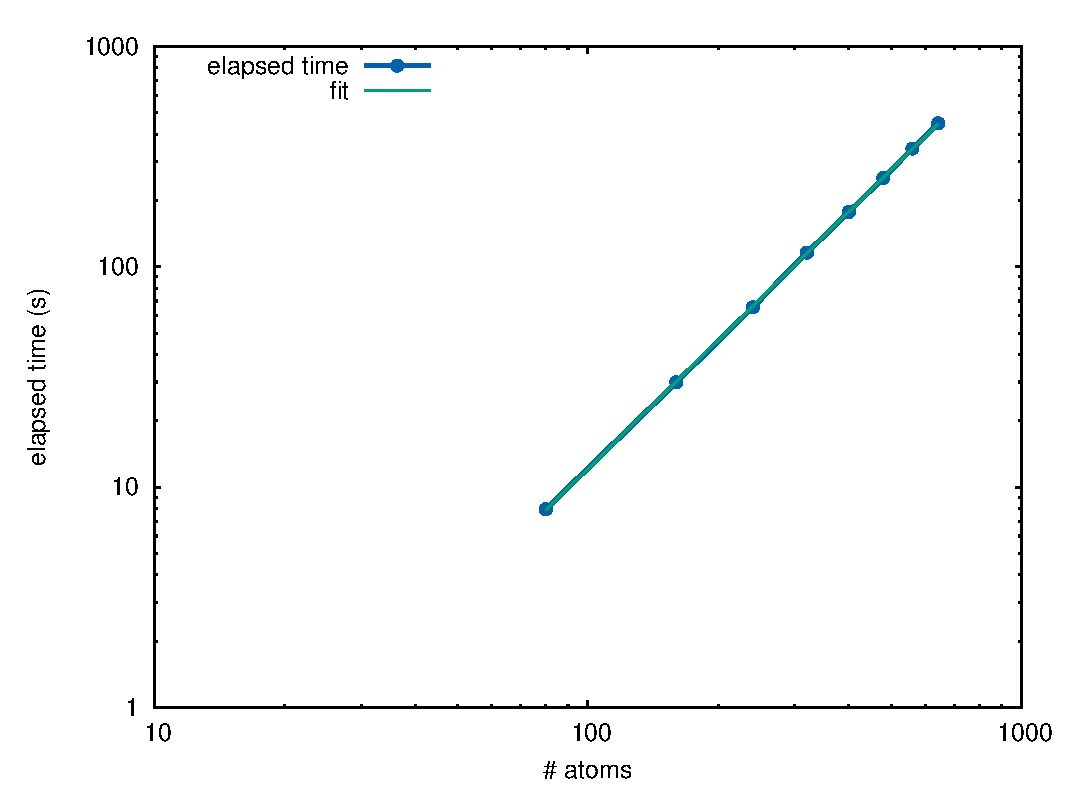
\includegraphics[width=0.6\textwidth]{serial.eps}
\end{figure}

The small discrepancy between the fitted exponent in Figure \ref{fig:serial}, i.e., 1.94, and the theoretical quadratic prediction can be justified in terms of the size of the tested systems, which fall into the pre-asymptotic, rather than asymptotic region. \color{red}To support this claim, we employed a second benchmark set (see table \ref{tab:set} for details), which includes a number of increasing size molecules and four additional systems obtained by incrementally considering the first four chains of a larger protein (PDB reference 2QHO). The computation of the ddPCM forces was performed using the shared-memory (OpenMP) parallel version of the code. 
\begin{table}
 \caption{Systems used to compute the scaling of the ddPCM forces. Peptide refers to a peptide formed by all 20 aminoacids. For 2QHO, the chains considered are reported in parentheses.\label{tab:set}}
 \begin{tabular}{lr}
  \toprule[0.1em] 
  Name or PDB reference & \# Atoms \\
  \midrule[0.05em]
  2RVD & 166 \\
  Ala25 & 259 \\
  Peptide & 328 \\
  2MLT (monomer) & 434 \\
  1EJG & 642 \\
  2QHO (A) & 1174 \\
  2QHO (AB) & 1921 \\
  2QHO (ABC) & 3152 \\
  2QHO (ABCD) & 3930 \\
  \bottomrule[0.1em]
 \end{tabular}
\end{table}
\color{black}
The timings are reported in figure \ref{fig:para}, and the fitted exponent, i.e., 1.98, supports our claim of asymptotic quadratic complexity. We remark that, overall, the observed timings are encouraging, despite the code not having been fully optimized. Nevertheless, the quadratic scaling makes the application of the ddPCM method to large systems challenging. 


\begin{figure}[t]
 \caption{Scaling of computation of the ddPCM forces (OpenMP parallel implementation). The results are plotted on a log-log scale, and fitted with a function of slope 1.99. The computations were performed on a dual Intel Xeon E5-2620 (v2) CPU cluster node (12 cores) equipped with 64 GB of RAM. Hyper-Threading was disabled.
\label{fig:para}}
 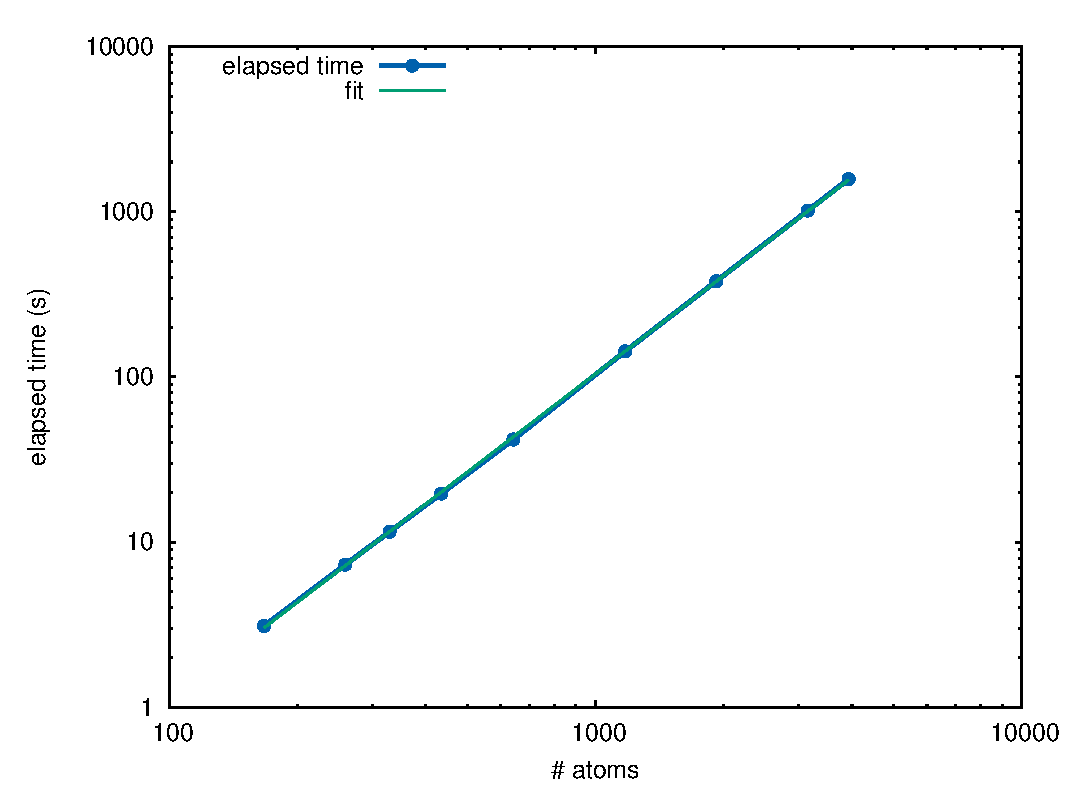
\includegraphics[width=0.6\textwidth]{paranew.eps}
\end{figure}


\section{Conclusions}\label{sec:conclusions}

In this paper we discussed analytical gradients of the electrostatic solvation energy arising from the Polarizable Continuum Model, discretized with a domain-decomposition strategy. The complete derivation is discussed in this paper, along with a quadratic complexity estimate, with respect to the number of atoms, that is supported by extensive numerical experiments.


The pilot implementation presented in this work is a stepping stone for future work. In fact, while the overall timings are acceptable and compare well to those obtained with different discretizations, the computational effort required by the solution of the ddPCM equations and the related forces is still large. This prevents to pursue applications on large and very large systems. In particular, while a more efficient implementation can be achieved and a better parallelization strategy implemented, the quadratic scaling of the computation cannot be circumvented. For this reason, a linear scaling implementation based on the use of the Fast Multipole Method is currently under investigation.

Finally, we have presented results for classical solutes only, i.e., solutes described by a classical force field. An implementation of ddPCM in the framework of quantum chemical methods is particularly attractive, since ddPCM shares with ddCOSMO the rigorous foundations, variational discretization and overall simplicity and limited number of parameters. Furthermore, the current quadratic scaling code already has a smaller constant than BEM-based discretizations. Indeed, those methods scale quadratically with respect to the number of total grid points, as opposed to ddPCM with scales linearly with respect to $N_\text{grid}$. As the systems that can be treated with quantum mechanical methods are well within reach of ddPCM, we expect the method to be already fully applicable in the framework of quantum Chemistry. 


\section*{Acknowledgments}
P.G.~and B.S.~acknowledge funding from the German Academic Exchange Service (DAAD) from funds of the ``Bundesministeriums f\"ur Bildung und Forschung'' (BMBF) for the project Aa-Par-T (Project-ID 57317909).
\appendix

\section{ddPCM discretization\label{app:pcm}}
The derivation of the ddPCM discretization employs the fact that the spherical harmonics $Y_\ell^m$ are eigenfunctions of the double layer operator $\cD_{0}$ on the unit sphere $\mathbb{S}$, i.e., $\cD_0 \, Y_\ell^m =  -2\pi/ (2\ell+1) \,  Y_\ell^m$, along with the following jump relation for the double layer potential
\begin{equation}\label{eq:jump}
	\lim_{\delta \to + 0} \big(\tilde{\cD}_0 \, Y_\ell^m\big)(y \pm \delta \nu) =  \pm 2\pi \, Y_\ell^m(y)+ ( \cD_0 \, Y_\ell^m )(y)
\end{equation}
where $\nu$ denotes the outward normal at $y \in \mathbb{S}$. We shall also rely on the invariance by translation and scaling of the double layer operator, namely  $(\mathcal{D}_j \, \Phi_{\varepsilon,j})(s) = (\mathcal{D}_0 \, \hat{\Phi}_{\varepsilon,j})(y)$, where $y = (s - x_j)/r_j$ and $\hat{\Phi}_{\varepsilon,j}$ is defined on $\mathbb{S}$ through the push-forward-like transformation $\hat{\Phi}_{\varepsilon,j}(y) = \Phi_{\varepsilon,j}(s)$. An analogous result holds for the double layer potential, namely $(\tilde{\cD}_k \, \Phi_{\varepsilon,k} )(x) = (\tilde{\cD}_0 \, \hat{\Phi}_{\varepsilon,j})(u)$ where $x \in \mathbb{R}^3 \setminus \overline{\Omega}_k$, $u = (x -x_j)/ r_j$, and $\tilde{\cD}_0$ is the double layer potential on $\mathbb{S}$.

As customary, in order to obtain a numerical discretization of \eqref{eq:1}, we multiply by a test function $\varphi$ and integrate over $\Gamma_j$
\begin{multline*}
\int_{\Gamma_j}\big( 2\pi \, g(\varepsilon_s) \, \Phi_{\varepsilon,j} - U_j \, {\mathcal{D}}_j \, \Phi_{\varepsilon,j} \big) \varphi +  \sum_{k \ne j} \, \int_{\Gamma_j} U_j \, \tilde{\mathcal{D}}_{k} \, \Phi_{\varepsilon,k} \, \varphi  = \\ 
= \int_{\Gamma_j}\big( 2 \pi \, {\Phi_j} - U_j \, {\mathcal{D}}_j \,\Phi_{j} \big) \varphi + \sum_{k \ne j} \,\int_{\Gamma_j } U_j \,  \tilde{\mathcal{D}}_{k} \, \Phi_{k}  \, \varphi
\end{multline*}
Here we isolated the diagonal terms for convenience.  Through the change of variable $y = (s- x_j)/r_j$, we obtain integrals over $\mathbb{S}$ which involve the hatted quantities, namely
\begin{multline}\label{eq:73}
 \int_{\mathbb{S}}\big( 2\pi \, g(\varepsilon_s) \, \hat{\Phi}_{\varepsilon,j} - \hat{U}_j \, {\mathcal{D}}_0 \, \hat{\Phi}_{\varepsilon,j} \big) \hat{\varphi} + \sum_{k \ne j} \,\int_{\mathbb{S}}  \hat{U}_j \, \tilde{\mathcal{D}}_0 \, \hat{\Phi}_{\varepsilon,k} \, \hat{\varphi}  = \\ 
= \int_{\mathbb{S}}\big( 2 \pi \, \hat{\Phi}_j - \hat{U}_j \, {\mathcal{D}}_0 \,\hat{\Phi}_j \big) \hat{\varphi} + \sum_{k \ne j} \, \int_{\mathbb{S}}  \hat{U}_j \, \tilde{\mathcal{D}}_0 \, \hat{\Phi}_{k}  \, \hat{\varphi}
\end{multline}
where we divided through by the surface Jacobian $r_j^2$.

In order to discretize the left-hand-side of the previous equation, we expand $\hat{\Phi}_{\varepsilon,j}$ as a series of spherical harmonics with coefficients $-[G_j]_{\ell'}^{m'}$, recall equation \eqref{eq:71}, and select as a test function $\hat{\varphi}$  the spherical harmonic $Y_{\ell}^{m}$. For the diagonal term, the orthogonality of the spherical harmonics, together with the fact that they are eigenfunctions of the double layer potential, yield
\begin{multline*}
 \int_{\mathbb{S}}\big( 2\pi \, g(\varepsilon_s) \, \hat{\Phi}_{\varepsilon,j} - \hat{U}_j \, {\mathcal{D}}_0 \, \hat{\Phi}_{\varepsilon,j} \big) Y_\ell^m = \\
= - 2 \pi  \, g(\varepsilon_s) \, \sum_{\ell',m'}  \, [G_j]_{\ell'}^{m'} \, \delta_{\ell \ell'} \delta_{mm'}  - \sum_{\ell',m'} \, [G_j]_{\ell'}^{m'} \, \frac{2\pi}{2\ell'+1} \int_{\mathbb{S}} \hat{U}_j \,  Y_{\ell'}^{m'}\, Y_\ell^m
\end{multline*}
The last step to obtain the diagonal block $A_{jj}^\varepsilon$ is to approximate the integral through a suitable quadrature formula with weights $\{w_n\}$ and nodes $\{ s_n\}$. Once the numerical quadrature is carried out and the spherical harmonics expansion is truncated at $\ell' = L_\text{max}$, we derive
\begin{equation}\label{eq:ajj}
[A_{jj}^\varepsilon]_{\ell \ell'}^{mm'} = 2\pi \, g(\varepsilon_s) %\frac{\varepsilon+1}{\varepsilon-1}
 \,  \delta_{\ell \ell'} \delta_{mm'} + \frac{2\pi}{2\ell'+1} \sum_{n=1}^{N_\text{grid}} \, w_n \, \hat{U}_j(s_n)  \, Y_{\ell'}^{m'}(s_n)\,  Y_\ell^m(s_n)
\end{equation}
which is the final expression of the diagonal block.

In order to discuss the off-diagonal blocks, let us write
\[
 \int_{\mathbb{S}} \hat{U}_j(y) \, (\tilde{\cD}_0 \, \hat{\Phi}_{\varepsilon,k})(u(y)) \, Y_{\ell}^{m}(y) \, dy = - \sum_{\ell',m'} \, [G_k]_{\ell'}^{m'} \,  \int_{\mathbb{S}} \hat{U}_j(y) \, (\tilde{\cD}_0 \, Y_{\ell'}^{m'})(u(y)) \, Y_{\ell}^{m}(y) \, dy 
\]
where we have explicitly indicated the variable of integration. We recall that, when $x \in \Gamma_j$, i.e., $x = s = x_j + r_j y$ for some $y \in \mathbb{S}$, then $u = u(y) = (x_j + r_j y -x_k)/r_k$. The function $\tilde{\cD}_0 \, Y_{\ell'}^{m'}$ is harmonic on $\mathbb{R}^3 \setminus \overline{B(0,1)}$, so that is has to coincide with the unique harmonic extension of its boundary value. The jump relation \eqref{eq:jump}, along with the eigenfunction property, provide the boundary value
\[
\lim_{\delta \; \to \; 0^+} \big(\tilde{\cD}_0 \, Y_{\ell'}^{m'}\big)(y + \delta \nu) =  2\pi \,Y_{\ell'}^{m'}(y)+ \big( \cD_0 \, Y_{\ell'}^{m'} \big)(y) = \frac{4 \pi \ell'}{2 \ell' + 1} \, Y_{\ell'}^{m'}(y)
\]
and, by elementary notions on harmonic functions, we conclude
\[
(\tilde{\cD}_0 \, Y_{\ell'}^{m'})(u) = \frac{4 \pi \ell'}{2 \ell' + 1} \, \frac{1}{|u|^{\ell' + 1}} \,  Y_{\ell'}^{m'}(u/|u|)
\]
After truncation the series expansion and performing numerical integration we obtain
\begin{equation}\label{eq:ajk}
[A_{jk}]_{\ell \ell'}^{m m'} =-  \frac{4 \pi \ell'}{2 \ell' + 1}  \sum_{n=1}^{N_\text{grid}} \, w_n  \,  \hat{U}_j(s_n) \, \frac{1}{|u(s_n)|^{\ell' + 1}} \, Y_{\ell'}^{m'}(u(s_n) / |u(s_n)|) \, Y_{\ell}^{m}(s_n)
\end{equation}
which is the final result.


The discretization of the right-hand-side of the ddPCM equation \eqref{eq:73} is entirely analogous. As a first step, we expand $\Phi_j$ as a series of spherical harmonics, recall \eqref{eq:71}, so that the orthogonality condition yields the following expression
\[
[F_j]_\ell^m = - \int_{\mathbb{S}} \hat{\Phi}_j \, Y_\ell^m= - \int_{\mathbb{S}} \hat{U}_j \, \hat{\Phi} \, Y_\ell^m(y)
\]
which is evaluated through numerical quadrature. The dependency of $F$ upon the nuclear positions in twofold. On one hand, the characteristic function $U_j$ depends upon $x_j$ and $x_i$ such that $i \in N_j$, see Appendix \ref{app:pcm_der}, so does $[F_j]_\ell^m$. On the other, the potential $\Phi$ itself depends on the nuclear positions. The derivation of the discrete operator $A_\infty$ arising from the right-hand-side is entirely analogous to the one described for the left-hand-side. In fact, it coincides with $A_\varepsilon$ with the natural extension $g(\infty) = 1$.
\section{ddCOSMO discretization \label{app:cosmo}}
As customary in a variational setting, we discretize equation \eqref{eq:2} by multiplying it with a test function $\varphi$ and integrating it over $\Gamma_j$. As a preliminary step, we manipulate the following integral as
\[
\int_{\Gamma_j} \tilde{\cS}_{jk} \, \sigma_k \, \varphi =\int_{\Gamma_j} n_j \, \tilde{\cS}_{k} \, \sigma_k \, \varphi = \int_{\Gamma_j} (1 - U_j ) \,n_j \, \tilde{\cS}_{k} \, \sigma_k \, \varphi = \int_{\Gamma_j} V_j \, \tilde{\cS}_{k} \, \sigma_k \, \varphi
\]
We inserted the characteristic function $U_j$ for convenience, and defined the rescaled characteristic function $V_j : \Gamma_j \to \mathbb{R}$ as $V(s) = (1 - U_j(s)) \, n_j(s)$. The reason for introducing the characteristic function is that we can modify it, e.g., replace it by a smooth counterpart, to improve robustness of the algorithm. We obtain the following variational formulation of the integral equation \eqref{eq:2}:
\[
\int_{\Gamma_j} \cS_j \, \sigma_j \, \varphi - \sum_{k \in N_j} \, \int_{\Gamma_j} V_j \, \tilde{\cS}_{k} \, \sigma_k \, \varphi= -\int_{\Gamma_j}  \Phi_{\varepsilon,j} \, \varphi %\qquad , \qquad j = 1, \ldots , M
\]
As a next step, we map quantities to the unit sphere $\mathbb{S}$. In order to do so, we employ the translation-invariant properties $(\cS_j \, \sigma_j)(s) = r_j( \cS_0 \, \hat{\sigma}_j)(z)$ and $(\tilde{\cS}_j \, \sigma_j)(x) = r_j( \tilde{\cS}_0 \, \hat{\sigma}_j)(u)$, where $\cS_0$ and $\tilde{\cS}_0$ are, respectively, the single layer operator and potential on the unit sphere, $y = (s - x_j)/r_j$, $u = (x - x_j)/r_j$, and $\hat{\sigma}_j(y) = \sigma_j(s)$. We obtain
\begin{equation}\label{eq:50}
r_j \int_{\mathbb{S}} \cS_0 \, \hat{\sigma}_j \, \hat{\varphi} - \sum_{k \in N_j} \, r_k  \int_{\mathbb{S}} \hat{V}_j \, \tilde{\cS}_0 \, \hat{\sigma}_k \, \hat{\varphi}= -\int_{\mathbb{S}}  \hat{\Phi}_{\varepsilon,j} \, \hat{\varphi}
\end{equation}
where we divided both sides by the surface Jacobian $r_j^2$. The workhorse for the objects $\cS_0 \, \hat{\sigma}_j$ and $\tilde{\cS}_0 \, \hat{\sigma}_k$ is the Addition Theorem for spherical harmonics.

If we expand $\hat{\sigma}_j$ through spherical harmonics $Y_\ell^m$ as
\[
\hat{\sigma}_j(y) = \frac{1}{r_j} \, \sum_{\ell'= 0}^{\infty} \sum_{m' = -\ell'}^{\ell'} \,  [X_j]_{\ell'}^{m'} \, Y_{\ell'}^{m'}(y)
\]
for some (unknown!)~coefficients $X_j = [X_j]_{\ell'}^{m'}$, the orthogonality property of the spherical harmonics implies
\[
(\cS_0 \, \hat{\sigma}_j)(y) = \frac{1}{r_j} \, \sum_{\ell'= 0}^{\infty} \sum_{m' = -\ell'}^{\ell'} \, \frac{4\pi}{2\ell' + 1}\, [X_j]_{\ell'}^{m'} \, Y_{\ell'}^{m'}(y)
\]
Thus, if we select as test functions the spherical harmonics, we obtain
\begin{equation*}%\label{eq:51}
r_j\int_\mathbb{S} \cS_0 \, \hat{\sigma}_j \, Y_\ell^m = \sum_{\ell'= 0}^{\infty} \sum_{m' = -\ell'}^{\ell'} \, \frac{4\pi}{2\ell' + 1} \, \delta_{\ell \ell'} \delta_{m m'}\, [X_j]_{\ell'}^{m'} 
\end{equation*}
due to their orthogonality. A numerical discretization is obtained by truncating the expansion for some $\ell'=L_\text{max}$. This provides the discrete action $L_{jj} \, X_j$, where the discrete operator
\begin{equation}\label{eq:61}
 [L_{jj}]_{\ell \ell'}^{m m'} =  \frac{4\pi}{2\ell' + 1} \, \delta_{\ell \ell'} \delta_{m m'}
\end{equation}
is diagonal and does not depend on the nuclear positions.

Analogously to the previous case, for the off-diagonal term the Addition Theorem implies
\[
(\tilde{\cS}_0 \, \hat{\sigma}_k)(u) = \frac{1}{r_k} \, \sum_{\ell'= 0}^{\infty} \sum_{m' = -\ell'}^{\ell'} \, \frac{4\pi}{2\ell' + 1}\, [X_k]_{\ell'}^{m'} \, |u|^{\ell'} \, Y_{\ell'}^{m'}(u/|u|)
\]
We relied on the fact that, when $x \in \Gamma_j$, i.e., $x = s = x_j + r_j y$, then $u = u(y) = (x_j + r_j y -x_k)/r_k$ and $|u| < 1$ because of the assumption $k \in N_j$. We obtain
\begin{multline*}
 r_k \int_\mathbb{S} \hat{V}_j(y) \, (\tilde{\cS}_0 \, \hat{\sigma}_k)(u(y)) \, Y_\ell^m(y) \, dy = \\
=  \sum_{\ell'= 0}^{\infty} \sum_{m' = -\ell'}^{\ell'} \, \frac{4\pi}{2\ell' + 1}\, [X_k]_{\ell'}^{m'} \int_\mathbb{S} \hat{V}_j(y) \, |u(y)|^{\ell'} \, Y_{\ell'}^{m'}(u(y)/|u(y)|) \, Y_\ell^m(y) \, dy
\end{multline*}
which, as opposed to the diagonal block $L_{jj}$, requires numerical integration.
%, so that
%\begin{equation}\label{eq:52}
%L_{jk} \, X_k = r_j^2 \, \sum_{\ell'= 0}^{L_\text{max}}  \sum_{m' = -\ell'}^{\ell'} \, \frac{4\pi}{(2\ell' + 1)}\, \sum_{n = 1}^{N_\text{grid}} w_n \, \hat{V}_j(s_n) \, |u(s_n)|^{\ell'} \, Y_{\ell'}^{m'}(u(s_n)/|u(s_n)|) \, Y_\ell^m(s_n)\, [X_k]_{\ell'}^{m'}  
%\end{equation}
This yields the off-diagonal block
\begin{equation}\label{eq:62}
[L_{jk}]_{\ell \ell'}^{m m'} =  \frac{4\pi}{2\ell' + 1}\, \sum_{n = 1}^{N_\text{grid}} w_n \, \hat{V}_j(s_n) \, |u(s_n)|^{\ell'} \, Y_{\ell'}^{m'}(u(s_n)/|u(s_n)|) \, Y_\ell^m(s_n)
\end{equation}
where we emploed a Lebedev grid with $N_\text{grid}$ nodes $\{s_n\}$ and weights $\{ w_n \}$ to perform numerical quadrature. We remark that the off-diagonal block $L_{jk}$ depends, \emph{a priori}, upon the nuclear positions $x_j$, $x_k$, and $x_i$, for $i \in N_j$.

When $\hat{\Phi}_{\varepsilon,j}$ is provided by the ddPCM step as a truncated series of spherical harmonics with coefficients $-[G_j]_{\ell'}^{m'}$, the discretization of the right-hand-side of \eqref{eq:50} becomes
\[
- \int_\mathbb{S} \hat{\Phi}_{\varepsilon,j} \, Y_\ell^m =  \sum_{\ell'= 0}^{L_\text{max}} \sum_{m' = -\ell'}^{\ell'} \, [G_j]_{\ell'}^{m'} \,  \int_{\mathbb{S}}  Y_{\ell'}^{m'} \, Y_\ell^m =  [G_j]_\ell^m
\]
because of the orthogonality condition. We conclude that, after the ddPCM step, the ddCOSMO step is simply $L \, X = G$.
 

% i.e., the load vector is simply
%\[
%[F_j]_\ell^m = - \int_\mathbb{S} \hat{\Phi}_{\varepsilon,j} \, Y_\ell^m
%\]
%which, in general, does require a numerical quadrature. However, when $\Phi_{\varepsilon,j}$ is provided by the ddPCM step as a truncated series of spherical harmonics with coefficients $-[G_j]_{\ell'}^{m'}$, the orthogonality condition implies
%\begin{equation*}
%[F_j]_\ell^m = - \int_\mathbb{S} \hat{\Phi}_{\varepsilon,j} \, Y_\ell^m =  \sum_{\ell'= 0}^{L_\text{max}} \sum_{m' = -\ell'}^{\ell'} \, [G_j]_{\ell'}^{m'} \,  \int_{\mathbb{S}}  Y_{\ell'}^{m'} \, Y_\ell^m =  [G_j]_\ell^m
%\end{equation*}
%so that we conclude that the load vector $F$ coincides with $G$ provided by the ddPCM step.
\section{Derivatives of ddPCM discretization}\label{app:pcm_der}

The function $U_j$ is, in practice, a smoothed version of the characteristic function. We use the following construction
\[
U_j(x_j + r_j y) =
\begin{cases}
1 - f_j(y) 	&\quad f_j(y) \le 1\\
0		&\quad \text{otherwise}
\end{cases}
\qquad , \qquad 
f_j(y) = \sum_{i \in N_j} \chi \bigg(\frac{|x_j + r_j y - x_i|}{r_i}\bigg)
\]
where $\chi$ is a regularized characteristic function of $[0,1]$. As previously, the variable $y$ varies on the unit sphere $\mathbb{S}$. This definition implies that $U_j$ depends upon the nuclear positions $x_j$ and $x_i$ such that $i \in N_j$.



Let $\{ s_n\}$ be $N_\text{grid}$ integration points, with associated weights $\{ w_n \}$, and define the following quantities
\[
t_n^{jk} = \frac{|x_j + r_j s_n -x_k|}{r_k} \qquad , \qquad s_n^{jk} = \frac{x_j + r_j s_n -x_k}{|x_j + r_j s_n -x_k|}%\quad , \quad U_j^n = U_j(x_j + r_j s_n)
\]
It is evident that $t_n^{jk}$ depends only upon the nuclear positions $x_j$ and $x_k$, as does $s_n^{jk}$. Standard differentiation yields
\begin{equation}\label{eq:75}
\nablaj t_n^{jk} = \frac{s_n^{jk}}{r_k} \qquad , \qquad \Dj \, s_n^{jk} = \frac{I - s_n^{jk} \otimes s_n^{jk} }{|x_j + r_j s_n - x_k|^3}
\end{equation}
where $I$ is the identity matrix and $\otimes$ indicates the outer product. We remark that the Jacobian matrix $\Dj \, s_n^{jk}$ is symmetric, and the ``twin'' relations $\nabla_{\! j} \, t_n^{jk} = - \nabla_{\! k} \, t_n^{jk}$ and $D_j \, s_n^{jk} = - D_k \, s_n^{jk}$ hold.

If we employ this notation and recall \eqref{eq:ajj} and \eqref{eq:ajk}, the blocks of the ddPCM operator can be written as
\begin{alignat*}{3}
{[A_{jj}^\varepsilon]}_{\ell \ell'}^{mm'}& = 2\pi \, g(\varepsilon_s) \, \delta_{\ell \ell'} \delta_{m m'}&& + \frac{2\pi}{2 \ell' + 1} \,\sum_{n= 1}^{N_\text{grid}} w_n \, \hat{U}_j(s_n)  \,Y_\ell^m(s_n) \,  Y_{\ell'}^{m'}(s_n) \\
{[A_{jk}^\varepsilon]}_{\ell \ell'}^{mm'}& =&& -  \frac{4 \pi \ell'}{2 \ell'+1} \, \sum_{n= 1}^{N_\text{grid}} w_n\, \hat{U}_j(s_n) \, Y_\ell^m(s_n) \, \big( t_n^{jk}\big)^{-(\ell'+1)} \, Y_{\ell'}^{m'} (s_n^{jk})
\end{alignat*}
The dependency of the diagonal block $A_{jj}^\varepsilon$ upon the nuclear positions occurs only through the characteristic function $U_j$. On the other hand, the off-diagonal block $A_{jk}^\varepsilon$ interacts with the nuclear positions through the characteristic function $U_j$, as well as $t_n^{jk}$ and $s_n^{jk}$. This implies that $\nablai A_{jj}$ is \emph{a priori} nonzero only when $i = j$ or $i \in N_j$. Similarly, $\nablai A_{jk}$ is \emph{a priori} nonzero only when $i = j$ or $i = k$ or $i \in N_j$.


The case of the diagonal blocks yields
\[
{[\nablai A_{jj}]}_{\ell \ell'}^{mm'} = \frac{2\pi}{2 \ell' + 1} \,\sum_{n=1}^{N_\text{grid}} w_n \, \nablai \hat{U}_j(s_n)  \,Y_\ell^m(s_n) \,  Y_{\ell'}^{m'}(s_n)
\]
so that only the derivatives of the characteristic function are required. The case of the off-diagonal blocks is significantly more involved, since it involves the gradient of the product of three functions, namely
\begin{equation}\label{eq:7}
{[\nablai A_{jk}]}_{\ell \ell'}^{mm'} = -  \frac{4 \pi \ell'}{2 \ell'+1} \, \sum_{n = 1}^{N_\text{grid}} w_n\, Y_\ell^m(s_n) \,\nablai \Big[ \hat{U}_j(s_n)  \,  \big( t_n^{jk}\big)^{-(\ell'+1)} \, Y_{\ell'}^{m'} (s_n^{jk}) \Big]
\end{equation}
We indicate the triple product as $I_{jk}$ and proceed to analyze its gradient when $i = j$, or $i = k$, or $i \in N_j \, , \, i \not= k$. Those three cases are mutually exclusive.

The case $i = j$ yields no simplification, and the gradient of the triple product has the three standard contributions, namely
\begin{multline}\label{eq:9}
\nablaj I_{jk}= \nablaj \hat{U}_j(s_n)  \,  \big( t_n^{jk}\big)^{-(\ell'+1)} \, Y_{\ell'}^{m'} (s_n^{jk}) \\
+ \hat{U}_j(s_n)  \, \nablaj \Big(  \big( t_n^{jk}\big)^{-(\ell'+1)} \Big) \, Y_{\ell'}^{m'} (s_n^{jk}) +  \hat{U}_j(s_n)  \,  \big( t_n^{jk}\big)^{-(\ell'+1)} \, \nablaj Y_{\ell'}^{m'} (s_n^{jk})
%\nablaj \Big[ \hat{U}_j(s_n)  \,  \big( t_n^{jk}\big)^{-(\ell'+1)} \, Y_{\ell'}^{m'} (s_n^{jk}) \Big] = \nablaj \hat{U}_j(s_n)  \,  \big( t_n^{jk}\big)^{-(\ell'+1)} \, Y_{\ell'}^{m'} (s_n^{jk}) \\
%- \hat{U}_j(s_n)  \, (\ell' + 1)  \big( t_n^{jk}\big)^{-(\ell'+2)} \, \nablaj t_n^{jk} \, Y_{\ell'}^{m'} (s_n^{jk}) + \hat{U}_j(s_n)  \,  \big( t_n^{jk}\big)^{-(\ell'+1)} \, \big( \Dj\, s_n^{jk} \big)^T\, \nablaj Y_{\ell'}^{m'} (s_n^{jk})
\end{multline}
In the implementation the differentiation is fully carried out through the chain rule, which employs the formulas \eqref{eq:75} for the derivatives of $t_n^{jk}$ and $s_n^{jk}$.

The case $i =k$ needs to be split into the subcases $k \in N_j$ and $k \not \in N_j$. The first subcase does not yield any simplification and reduces to \eqref{eq:9}. On the other hand, when $k \not\in N_j$, the first term on the right-hand-side of \eqref{eq:9} drops out, and we obtain
\[
\nablak I_{jk} = 
 \hat{U}_j(s_n)  \, \nablak \Big(  \big( t_n^{jk}\big)^{-(\ell'+1)} \Big) \, Y_{\ell'}^{m'} (s_n^{jk}) +  \hat{U}_j(s_n)  \,  \big( t_n^{jk}\big)^{-(\ell'+1)} \, \nablak Y_{\ell'}^{m'} (s_n^{jk})
\]

Finally, when $i \in N_j$ and $i \not=k$ the second and third term on the right-hand-side of \eqref{eq:9} vanish, and we obtain 
\[
\nablai I_{jk} = \nablaj \hat{U}_j(s_n)  \,  \big( t_n^{jk}\big)^{-(\ell'+1)} \, Y_{\ell'}^{m'} (s_n^{jk})
\]

This conclude our discussion on the derivative of the PCM matrix, we remark that $\nablai A_{jk}$ is \emph{a priori} nonzero only when $i \in N_j \cup \{ j,k\}$.


%%\cdots\Big[ \nabla U_j^n  \,  \big( t_n^{jk}\big)^{-(\ell'+1)} \, Y_{\ell'}^{m'} (s_n^{jk}) + U_j^n  \, \nabla \Big( \big( t_n^{jk}\big)^{-(\ell'+1)} \Big)\, Y_{\ell'}^{m'} (s_n^{jk}) + U_j^n  \,  \big( t_n^{jk}\big)^{-(\ell'+1)} \, \nabla Y_{\ell'}^{m'} (s_n^{jk}) \Big]
%%\end{multline*}
%However, since $t_n^{jk}$ and $s_n^{jk}$ depend only upon $x_j$ and $x_k$, if we assume $i \not=j$ and $i\not=k$, we obtain
%\begin{equation}\label{eq:8}
%{[\nablai A_{jk}]}_{\ell \ell'}^{mm'} = -  \frac{4 \pi \ell'}{2 \ell'+1} \, \sum_{n} w_n\, Y_\ell^m(s_n) \,\nablai U_j^n  \,  \big( t_n^{jk}\big)^{-(\ell'+1)} \, Y_{\ell'}^{m'} (s_n^{jk})
%\end{equation}
%%Such relation holds, in particular, for $i \in N_j$ and $i \not= k$.
%Thus, since $U_j^n$ depends only upon $x_i$ if $i \in N_j$ or $i=j$, we conclude that $\nablai A_{jk}$ vanishes whenever $i \not= j$ and $i \not=k$ and $i \not\in N_j$. In order to discuss the opposite case, i.e., $i = j$ or $i =k$ or $i \in N_j$, notice that the events $(i = j)$ and $(i = k)$ are mutually exclusive, as are $(i = j)$ and $(i \in N_j)$. We obtain the three subcases $i = j$, and $i = k$, and $i \in N_j \, , \, i \not= k$, which will be addressed individually.
%
%Standard differentiation implies that
%\begin{multline}\label{eq:9}
%\nablai \Big[ U_j^n  \,  \big( t_n^{jk}\big)^{-(\ell'+1)} \, Y_{\ell'}^{m'} (s_n^{jk}) \Big] = \nablai U_j^n  \,  \big( t_n^{jk}\big)^{-(\ell'+1)} \, Y_{\ell'}^{m'} (s_n^{jk}) \\
%- U_j^n  \, (\ell' + 1)  \big( t_n^{jk}\big)^{-(\ell'+2)} \, \nablai t_n^{jk} \, Y_{\ell'}^{m'} (s_n^{jk}) + U_j^n  \,  \big( t_n^{jk}\big)^{-(\ell'+1)} \, \big( \Di\, s_n^{ji} \big)^T\, \nablai Y_{\ell'}^{m'} (s_n^{jk})
%\end{multline}
%where $\Di$ emphasizes that the gradient of the vector quantity $s_j^{jk}$ is indeed its Jacobian matrix and where the extra subscripts refer to the variables with respect to which differentiation is taken. We proceed to evaluate $\nablai t_n^{jk}$ and $ \Di \, s_n^{jk}$. When $i = j$, differentiation implies
%\[
%\nablaj t_n^{jk} = \frac{s_n^{jk}}{r_k} \qquad , \qquad \Dj \, s_n^{jk} = \frac{I - s_n^{jk} \otimes s_n^{jk} }{|x_j + r_j s_n - x_k|^3}
%\]
%where $I$ is the identity matrix and $\otimes$ indicates the outer product. We remark that the Jacobian matrix $\Dj \, s_n^{jk}$ is symmetric, so that the transpose in \eqref{eq:9} is redundant. 
%Due to the particular relation between $x_j$ and $x_k$, we obtain $\nabla_{\! j} \, t_n^{jk} = - \nabla_{\! k} \, t_n^{jk}$ and $D_j \, s_n^{jk} = - D_k \, s_n^{jk}$.
%We can therefore analogously derive the case $i = k$ and those relationships imply
%\begin{multline*}
%\nabla_{\! j} \Big[ U_j^n  \,  \big( t_n^{jk}\big)^{-(\ell'+1)} \, Y_{\ell'}^{m'} (s_n^{jk}) \Big] + \nabla_{\! k} \Big[ U_j^n  \,  \big( t_n^{jk}\big)^{-(\ell'+1)} \, Y_{\ell'}^{m'} (s_n^{jk}) \Big] = \\
%  \Big[ \nabla_{\! j} \, U_j^n + \nabla_{\! k} \, U_j^n  \Big]  \big( t_n^{jk}\big)^{-(\ell'+1)} \, Y_{\ell'}^{m'} (s_n^{jk})
%\end{multline*}
%which provide a convenient way of evaluating $[\nabla_{\! k} \, A_{jk}]_{\ell \ell'}^{m m'}$ from $[\nabla_{\! j} \, A_{jk}]_{\ell \ell'}^{m m'}$. In fact, we obtain the quasi-skew-symmetric relation
%\[
%[ \nabla_{\! j} \, A_{jk}]_{\ell \ell'}^{m m'} + [\nabla_{\! k} \, A_{jk}]_{\ell \ell'}^{m m'} = -  \frac{4 \pi \ell'}{2 \ell'+1} \, \sum_{n} w_n\, Y_\ell^m(s_n) \Big[ \nabla_{\! j} \, U_j^n + \nabla_{\! k} \, U_j^n  \Big]  \big( t_n^{jk}\big)^{-(\ell'+1)} \, Y_{\ell'}^{m'} (s_n^{jk})
%\]
%for $\nablai A_{jk}$. Finally, the case $i \in N_j \, , \, i \not= k$ reduces to \eqref{eq:8}.
% Ben's notes
%\noindent
{\bf A quick overview of sparsity of $\nablai A_{jk}$}: There is nothing new, but should clarify a bit the computational complexity of computing the forces.
\begin{itemize}
\item {\bf Diagonal terms: $j=k$:}
	\begin{itemize}
		\item If $i\in N_j=N_k$ or $i=j=k$, then $[ \nablai A_{jj}]_{\ell \ell'}^{m m'} \neq 0$. 
		\item If $i\not \in N_j=N_k$ and  $i\neq j=k$, then $[ \nablai A_{jk}]_{\ell \ell'}^{m m'} = 0$.
	\end{itemize}
\item {\bf Off-diagonal terms: $j\neq k$:}
	\begin{itemize}
		\item If $i=k$, then $[ \nablai A_{jk}]_{\ell \ell'}^{m m'} \neq 0$.
		\item If $i=j$, then $[ \nablai A_{jk}]_{\ell \ell'}^{m m'} \neq 0$.
		\item If $i\neq j$ and $i\neq k$
		\begin{itemize}
			\item If $i\in N_j$ and $i\neq k$, then $[ \nablai A_{jk}]_{\ell \ell'}^{m m'} \neq 0$.
			\item If $i\not\in N_j$ and $i\neq k$, then $[ \nablai A_{jk}]_{\ell \ell'}^{m m'} =0 0$.
		\end{itemize}
	\end{itemize}
\end{itemize}
From a different perspective, we want now to analyse the complexity of the matrix-vector product $\nablai A f$ for some vector $f$.
%

We see that 
\begin{align*}
	[(\nablai A f)_j]_\ell^m 
	&= \sum_k \sum_{\ell',m'} [\nablai A_{jk}]_{\ell \ell'}^{m m'} [f_k]_{\ell'}^{m'} \\
	&= \sum_{\ell',m'} [\nablai A_{jj}]_{\ell \ell'}^{m m'} [f_j]_{\ell'}^{m'} 
	+ \sum_{k\neq j} \sum_{\ell',m'} [\nablai A_{jk}]_{\ell \ell'}^{m m'} [f_k]_{\ell'}^{m'} 
\end{align*}
so that we split $\nablai A$ into the block-diagonal part $\nablai A_d$ and the off-diagonal part $\nablai A_o$.
\begin{align*}
	[(\nablai A_d f)_j]_\ell^m 
	&= \sum_{\ell',m'} [\nablai A_{jj}]_{\ell \ell'}^{m m'} [f_j]_{\ell'}^{m'} \\
	[(\nablai A_o f)_j]_\ell^m 
	&= \sum_{k\neq j} \sum_{\ell',m'} [\nablai A_{jk}]_{\ell \ell'}^{m m'} [f_k]_{\ell'}^{m'} 
\end{align*}
For the diagonal part, we have that
\[
	[(\nablai A_d f)_j]_\ell^m = 0
\]
if $i\not\in N_j$ and $i\neq j$. For a fixed $i$, the number of non-zero contributions (indexed by $j$) from the diagonal is independent of $M$. $\mathcal O(1)$

For the off-diagonal part, we distinguish three cases.

Case 1 ($i=j$ and necessarily $i\neq N_j$):
\[
	[(\nablai A_o f)_i]_\ell^m 
	= 	\sum_{k\neq i} \sum_{\ell',m'} [\nablai A_{ik}]_{\ell \ell'}^{m m'} [f_k]_{\ell'}^{m'} 
\]
Here, all terms $k\neq i$ must be considered. This operation is $\mathcal O(M)$ but this case happens for one $j$ only.

Case 2 ($i\neq j$ and $i\in N_j$):
\[
	[(\nablai A_o f)_j]_\ell^m 
	= \sum_{\ell',m'} [\nablai A_{ji}]_{\ell \ell'}^{m m'} [f_i]_{\ell'}^{m'} 
	+ \sum_{k\neq j, k\neq i} \sum_{\ell',m'} [\nablai A_{jk}]_{\ell \ell'}^{m m'} [f_k]_{\ell'}^{m'} 
\]
This operation is $\mathcal O(M)$, but this case happens for $\mathcal O(1)$ values of $j$ only.

Case 3 ($i\neq j$ and $i\not \in N_j$):
\[
	[(\nablai A_o f)_j]_\ell^m 
	= \sum_{\ell',m'} [\nablai A_{ji}]_{\ell \ell'}^{m m'} [f_i]_{\ell'}^{m'} 
\]
This operation is $\mathcal O(1)$ and this needs to be done for $\mathcal O(M)$ values of $j$.

Therefore, we see that computing all coefficients of the matrix-vector product $[(\nablai A f)_j]_\ell^m $ for one fixed $i$ requires $\mathcal O(M)$ of operations. 
Now, this needs to be done for each $i=1,\ldots,M$ such that the overall complexity to compute all coefficients $[(\nablai A f)_j]_\ell^m $ for all $i$ and $j$ is $\mathcal O(M^2)$.



%1. Use that $\nablai A_\infty=\nablai A_\varepsilon$ and that $L \, X=G$:
%\begin{alignat*}{1}
%h_i &= \nablai A_\infty \, F +  A_\infty \, \nablai F - \nablai A_\varepsilon \, L \, X -  A_\varepsilon \, \nablai L \, X\\
%&= \nablai A \, (F-  G) +  A_\infty \, \nablai F  -  A_\varepsilon \, \nablai L \, X
%\end{alignat*}
%
%2. Explain how to do the following operations efficiently:
%\begin{alignat*}{3}
%\langle s, \nablai A \, (F-  G) \rangle &= \langle (\nablai A)^* \, s,  F-  G \rangle ? \\
%\langle s, A_\infty \, \nablai F \rangle &= \langle A_\infty \,^* \, s,  \nablai F \rangle \\
%\langle s, A_\varepsilon \, \nablai L \, X \rangle &= \langle (A_\varepsilon\, \nablai L)^* \, s,  X \rangle ? \\
%\end{alignat*}
%I don't see how the first and third term are efficiently done in practice?
%
%3. Use the skew-symmetric relationship from above.



\bibliography{biblio}
\end{document}
